\documentclass{amsart}

\usepackage{amsmath}
\usepackage{amssymb}
\usepackage{mathrsfs}
%\usepackage{amscd}
\usepackage{stmaryrd}


%\usepackage[mathscr]{eucal}

\usepackage{hyperref}
\usepackage{enumitem}

%\usepackage{booktabs,caption}
%\usepackage{longtable}

%\usepackage[english]{babel}
\usepackage[british]{babel}
\usepackage[all]{xy}
\usepackage{comment}
\usepackage{graphicx}
%\usepackage{color}
%\usepackage[all,cmtip]{xy}
\usepackage{caption}
\usepackage{subcaption}
\usepackage{xcolor}
\usepackage{tikz}
\usetikzlibrary{cd}

%bibliografia

%\usepackage{amsrefs}
%\usepackage[abbrev]{amsrefs}
%\usepackage[alphabetic]{amsrefs}
%\usepackage[alphabetic,nobysame]{amsrefs}
%\usepackage{cite}
\usepackage[abbrev]{amsrefs}





%ambienti teoremi
%\theoremstyle{theorem}
\newtheorem{theorem}{Theorem}[section]
\newtheorem{lemma}[theorem]{Lemma}
\newtheorem{prop}[theorem]{Proposition}
\newtheorem{cor}[theorem]{Corollary}
%\newtheorem{conj}[theorem]{Conjecture}
\newtheorem{question}[theorem]{Question}
%\newtheorem{claim}[theorem]{Claim}

%main theorem
%\newtheorem{maintheorem}{Theorem}
%\renewcommand*{\themaintheorem}{\Alph{maintheorem}}

%ambienti definizioni
\theoremstyle{definition}
%\newtheorem{definition}[theorem]{Definition}
\newtheorem{remark}[theorem]{Remark}
%\newtheorem{notation}[theorem]{Notation}
\newtheorem{example}[theorem]{Example}
%\newtheorem{setup}[theorem]{Setup}
%\newtheorem{construction}[theorem]{Construction}

\numberwithin{equation}{section}

%standard commands

\newcommand{\Kps}[2]{M^\mathrm{Kps}_{#1, #2}}
\newcommand{\Kss}[2]{\mathcal{M}^\mathrm{Kss}_{#1, #2}}
\newcommand{\modulismooth}{M_{\rho=4}^\mathrm{sm}}

%general symbols
\renewcommand{\setminus}{\smallsetminus}
\renewcommand{\emptyset}{\varnothing}
%\newcommand{\epsi}{\varepsilon}
%\newcommand{\phiv}{\varphi}
%\newcommand{\epsi}{\varepsilon}
%\newcommand{\inv}{^{-1}}
\newcommand{\into}{\hookrightarrow} %monomorfismo
\newcommand{\onto}{\twoheadrightarrow} %epimorfismo
\newcommand{\id}{\mathrm{id}} %identita`
%\def\der#1#2{\frac{\partial #1}{\partial #2}} %derivata parziale
%\newcommand{\GL}{\mathrm{GL}} %general linear group
%\DeclareMathOperator{\coker}{coker}
%\DeclareMathOperator{\rank}{rank}
%\DeclareMathOperator{\embdim}{embdim}
\newcommand{\Gm}{\mathbb{G}_\mathrm{m}}
\newcommand{\al}{\alpha}

%general algebraic geometry symbols
%\DeclareMathOperator\Aut{Aut}
%\DeclareMathOperator{\Sing}{Sing}
%\DeclareMathOperator{\spe}{sp}
\DeclareMathOperator{\Hom}{Hom} %spazio degli omomorfismi
%\DeclareMathOperator{\RHom}{RHom} %spazio degli omomorfismi
%\newcommand{\Ext}{\mathrm{Ext}}
%\newcommand{\cExt}{\mathcal{E}xt}
\newcommand{\cHom}{\mathcal{H}om}
%\newcommand{\SSpec}{\mathbf{Spec}}
%\newcommand{\cSym}{\mathcal{S}ym}
\DeclareMathOperator{\Spec}{Spec} %spettro di un anello
\DeclareMathOperator{\Spf}{Spf} % formal spectrum
%\DeclareMathOperator{\Proj}{Proj} %spazio proiettivo
\DeclareMathOperator{\Pic}{Pic}
\DeclareMathOperator{\Cl}{Cl}
\DeclareMathOperator{\Div}{Div}
\DeclareMathOperator{\conv}{conv}
\DeclareMathOperator{\Aut}{Aut}
\DeclareMathOperator{\SL}{SL}
\DeclareMathOperator{\GL}{GL}
\newcommand{\git}{/ \! \!  /}

%\newcommand{\bmu}{\boldsymbol{\mu}}

%\def\HilbS#1{\mathrm{Hilb}( #1 , -K_{#1})}
%\def\pow#1{[ \! \ [ #1 ] \! ] }
\def\pow#1{ \llbracket  #1 \rrbracket }

\newcommand{\LH}[1]{\marginpar{\footnotesize \color{blue} {\colorbox{green!20}{{\bf {TODO}}}: {#1}}}}

\newcommand{\Def}[1]{\mathrm{Def}_{#1}}

%\newcommand{\conv}[1]{\mathrm{conv}\left( #1 \right)}
\newcommand{\cone}[1]{\mathrm{cone}\left( #1 \right)}

%%%%%%%%%%%%%%%%%%%%%%%

%alphabets

%calligrafico maiuscolo
%\newcommand\cB{\mathcal{B}}
%\newcommand\cD{\mathcal{D}}
%\newcommand\cE{\mathcal{E}}
\newcommand\cF{\mathcal{F}}
%\newcommand\cG{\mathcal{G}}
%\newcommand\cH{\mathcal{H}}
%\newcommand\cI{\mathcal{I}}
%\newcommand\cL{\mathcal{L}}
%\newcommand\cM{\mathcal{M}}
\newcommand\cO{\mathcal{O}}
%\newcommand\cR{\mathcal{R}}
%\newcommand\cS{\mathcal{S}}
\newcommand\cX{\mathcal{X}}
\newcommand\cU{\mathcal{U}}
%\newcommand\cV{\mathcal{V}}


%veramente calligrafico
%\newcommand\cT{\mathscr{T}}
%\newcommand\scrX{\mathscr{X}}
%\newcommand\scrY{\mathscr{Y}}
%\newcommand\scrZ{\mathscr{Z}}

%grassetto matematico maiuscolo
\renewcommand\AA{\mathbb{A}}
\newcommand\CC{\mathbb{C}}
\newcommand\FF{\mathbb{F}}
\newcommand\GG{\mathbb{G}}
\newcommand\HH{\mathbb{H}}
%\newcommand{\KK}{\mathbb{K}}
\newcommand{\KK}{\Bbbk}
%\newcommand{\LL}{\mathbb{L}}
\newcommand\NN{\mathbb{N}}
\newcommand\PP{\mathbb{P}}
\newcommand\QQ{\mathbb{Q}}
\newcommand\RR{\mathbb{R}}
\newcommand\TT{\mathbb{T}}
\newcommand\ZZ{\mathbb{Z}}

%dritto maiuscolo
%\newcommand\rG{\mathrm{G}}
\newcommand\rH{\mathrm{H}}
%\newcommand\rL{\mathrm{L}}
\newcommand\rN{\mathrm{N}}
%\newcommand\rR{\mathrm{R}}
%\newcommand{\rT}{\mathrm{T}}
%\newcommand\rV{\mathrm{V}}

%dritto minuscolo
\newcommand\rmm{\mathrm{m}}

%gotico minuscolo
%\newcommand{\frakm}{\mathfrak{m}}
%\newcommand{\frakp}{\mathfrak{p}}

%gotico maiuscolo
%\newcommand{\frakX}{\mathfrak{X}}
%\newcommand{\frakY}{\mathfrak{Y}}


% Use uppercase letters for sub-figure numbering (A, B, ... instead of a, b, ...)
% (Per default \thesubfigure is defined as \alph{subfigure}, i.e. lowercase letters)
\renewcommand\thesubfigure{\Alph{subfigure}}

\newcommand{\arxiv}[1]{\href{https://arxiv.org/abs/#1}{\textsf{arXiv:#1}}}

%%%%%%%%%%%%%%


\title[On K-moduli of Fano threefolds with degree 28 and Picard rank 4]{On K-moduli of Fano threefolds \\ with degree 28 and Picard rank 4}



\author{Liana Heuberger}
\address{Department of Mathematical Sciences, University of Bath, Claverton Down, Bath, BA2 7AY, United Kingdom}
\email{lh2457@bath.ac.uk}

\author{Andrea Petracci}
\address{Dipartimento di Matematica, Universit\`a di Bologna, Piazza di Porta San~Donato 5, Bologna, 40126, Italy}
\email{a.petracci@unibo.it}





%\usepackage{showlabels}




\begin{document}
	

\begin{abstract}
We analyse the local structure of the K-moduli space of Fano varieties at a toric singular K-polystable Fano $3$-fold, which deforms to smooth Fano $3$-folds with anticanonical volume $28$ and Picard rank $4$. In particular, by constructing an algebraic deformation of this toric singular Fano, we show that the irreducible component of K-moduli parametrising these smooth Fano $3$-folds is a rational surface.
\end{abstract}

\maketitle



\section{Introduction}



\subsection{Context}

We work over $\CC$.  In the study of Fano varieties \emph{K-stability} \cite{tian_KE, donaldson_stability}  has become a fundamental topic in recent years, for two main reasons: it is the algebraic counterpart of the existence of K\"ahler--Einstein metrics \cite{chen_donaldson_sun,tian_KstabKE}, and it has allowed to construct projective moduli spaces for Fano varieties.

More precisely, by \cite{ABHLX,BLX,properness_K_moduli,blum_xu_uniqueness,jiang_boundedness,lwx,projectivity_K_moduli_final,xu_minimizing,xu_zhuang}, for every positive integer $n$ and for every positive rational number $v$, there exists a projective scheme $\Kps{n}{v}$ over $\CC$, whose closed points are in a natural one-to-one correspondence with the K-polystable Fano varieties $X$ of dimension $n$ and anticanonical volume $v$. This is called a \emph{K-moduli space}. We refer the reader to \cite{xu_survey} for a survey on this topic.

An important problem is to decide if a given Fano variety is K-(semi/poly)stable: this is the \emph{Calabi problem}.
For smooth del Pezzo surfaces this has been completely solved in \cite{tian_del_pezzo}.
For the general member of the 105 deformation families of smooth Fano $3$-folds, the Calabi problem has been solved in \cite{calabi_problem_book}.
For all (not necessarily general) smooth Fano 3-folds there is much recent and ongoing work, e.g.\ \cite{liu_rank2, cheltsov_denisova_fujita, cheltsov_park, cheltsov_fujita_kishimoto_okada, denisova, belousov_loginov}.
Other smooth Fano varieties are studied in \cite{zhuang, abban_zhuang}.

It is natural to investigate the geometry of K-moduli spaces of Fano varieties.
Only few cases are known, e.g.\ smooth del Pezzo surfaces  \cite{mabuchi_mukai,odaka_spotti_sun}, cubic $3$-folds \cite{liu_xu} and cubic $4$-folds \cite{liu_cubic_fourfolds}.

Here we present results about a specific family of smooth Fano $3$-folds by using toric geometry and deformation theory techniques which originate in mirror symmetry \cite{ccggsk}.

\subsection{The family \textnumero4.2}
There is only one deformation family of smooth Fano $3$-folds with Picard rank $4$ and anticanonical volume $28$: this is the $2$nd entry in the Mori--Mukai list \cite{MM82,MM03} (and also in \cite{iskovskikh_prokhorov}) of families of smooth Fano $3$-folds with Picard rank $4$, thus it is denoted by \textnumero4.2 in \cite{calabi_problem_book}.
This family is denoted by $\mathrm{MM}_{4-3}$ in \cite[\S87]{quantum_periods} because the authors have reordered the families of smooth Fano $3$-folds of Picard rank $4$ so that the anticanonical volume increases along the list.
The other invariants of this family are $h^{1,2}(X) = 1$ and $\chi(T_X) = -1$.

Each member of the family \textnumero4.2 is the blow-up of the cone over a smooth quadric surface $S \subset \PP^3$ with centre the disjoint union of the vertex and an elliptic curve on $S$.
Each member of the family \textnumero4.2 is K-polystable by \cite{calabi_problem_book}, hence gives a point in $\Kps{3}{28}$, which is the K-moduli space of $3$-dimensional K-polystable Fano varieties with anticanonical volume $28$.

We prove the following:

\begin{theorem}\label{thm:main}
	Let $M = \Kps{3}{28}$ be the K-moduli space of K-polystable Fano $3$-folds with anticanonical volume $28$.
	Let $\modulismooth \subset M$ be the locus which parametrises the smooth K-polystable Fano $3$-folds with anticanonical volume $28$ and Picard rank $4$.
	
	Then there exists an open subscheme $U$ of $M$ such that $U$ is a smooth rational surface, $U \cap \modulismooth \neq \emptyset$ and $U \setminus \modulismooth$ is a smooth rational curve.
\end{theorem}

We therefore conclude that the irreducible component of $\Kps{3}{28}$ containing $\modulismooth$ is a rational surface. 

\subsection{Idea of the proof}

We pick a singular K-polystable toric Fano $3$-fold $X$ whose singular locus consists of $4$ ordinary double points.
In \cite[\S5.1]{ask_petracci} it is shown that the $3$-fold $X$ deforms to the members of the family \textnumero4.2 and the base space of the miniversal deformation of $X$ is a polydisc of dimension $4$. 
However, no information about the local structure, in the Zariski topology, of the K-moduli space can be derived from this infinitesimal study.

Here, we construct an explicit algebraic model of the miniversal deformation of $X$ over a Zariski neighbourhood of the origin in the affine space $\AA^4$, i.e.\ we exhibit a flat algebraic deformation of $X$ over $\AA^4$ such that its  formal completion at the origin is the miniversal deformation of $X$.

To achieve this we use the Laurent inversion method introduced in \cite{laurent_inversion} and used to systematically construct (not necessarily smooth) Fano 3-folds in \cite{from_cracked_to_fano,Heuberger_QFLI}.
Indeed, we find a toric $4$-fold $F$ such that $X$ is a divisor in $F$ and we are able to smooth $X$ by deforming it inside the linear system $\vert \cO_F(X) \vert$. We then show that this algebraic deformation induces the miniversal one.

We deduce that the K-moduli space is unirational near the point $[X]$ corresponding to $X$.
Moreover, by using deformation-theoretic techniques in Proposition~\ref{prop:definition_P_X}(8)  we show that the K-moduli space is smooth of dimension $2$ at $[X]$.
This proves the rationality in the statement.


\begin{remark}
	Following a suggestion of Ivan Cheltsov, it is likely that there exists an alternative way to prove the rationality of the irreducible component of $\Kps{3}{28}$ containing to the points corresponding the members of the family \textnumero4.2.
	Indeed, by using their birational description, one should be able to prove that there exists a dominant rational map from the linear system $\vert \cO_{\PP^1 \times \PP^1}(2,2) \vert$ to the irreducible component of $\Kps{3}{28}$ that we consider.	
	
	However, the rationality and the (local) smoothness of the curve $U\setminus \modulismooth$ inside $\Kps{3}{28}$ parametrising singular Fano $3$-folds near our toric Fano $3$-fold $X$ can be proved only by analysing the deformation theory of $X$, which is exactly what we have done.
\end{remark}

\begin{remark}
	We expect that there exists a toric Fano $3$-fold $X'$ with Gorenstein singularities which deforms to two different families of smooth Fano $3$-folds, namely \textnumero4.2 (which is the family studied in this paper) and \textnumero2.21 (which is the family consisting of the blowups of the smooth quadric $3$-fold at a twisted quartic curve). Both families have anticanonical volume $28$, but they have different Betti numbers. The general member of the family  \textnumero2.21 is K-polystable \cite{calabi_problem_book}.
	
	Unfortunately, the singular toric Fano $3$-fold $X'$, which is expected to have the properties above, is not K-semistable.
	It is therefore natural to wonder whether the two irreducible components of $\Kps{3}{28}$ generically parametrising K-polystable members of the families \textnumero2.21 and \textnumero4.2 belong to the same connected component of $\Kps{3}{28}$.
\end{remark}

\subsection*{Notation and conventions} \label{sec:notation}
The set of non-negative (resp.\ positive) integers is denoted by $\NN$ (resp.\ $\NN^+$).
We work over an algebraically closed field of characteristic zero, denoted by $\CC$.
%Every ring is commutative with identity.
Every toric variety or toric singularity is assumed to be normal.
%A polygon is by definition a polytope of dimension $2$.
A Fano variety is a normal projective variety whose anticanonical divisor is $\QQ$-Cartier and ample.
A del Pezzo surface is a Fano variety of dimension $2$.

%For the names of the deformation families of smooth Fano $3$-folds we follow the conventions of \cite{quantum_periods_Fano_3folds}.
%The symbol $V_d$ denotes the deformation family of smooth Fano $3$-folds of Picard rank $1$, Fano index $1$ and anticanonical degree $d$.
%The symbol $B_d$ denotes the deformation family of smooth Fano $3$-folds of Picard rank $1$, Fano index $2$ and anticanonical degree $8d$.
%For $2 \leq \rho \leq 10$, the symbol \morimukai{\rho}{k} denotes the $k$th entry in the Mori--Mukai list \cite{MM82, MM86,MM03} of smooth Fano $3$-folds of Picard rank $\rho$, with the exception of the case $\rho = 4$, where we place the $13$th entry in Mori and Mukai's rank-4 list in between the first and the second elements of that list.
%This reordering ensures that, for each $\rho \geq 2$, the sequence \morimukai{\rho}{1}, \morimukai{\rho}{2}, \morimukai{\rho}{3}, ... is in order of increasing degree.

\subsection*{Acknowledgements}
LH would like to thank Tom Coates and Al Kasprzyk for many conversations during the preparation of \cite{Heuberger_QFLI}, which has proved to be a comprehensive testing ground for $3$-fold Laurent inversion. AP wishes to thank Ivan Cheltsov and Anne-Sophie Kaloghiros for many fruitful conversations.

LH is supported by Leverhulme grant RPG-2021-149.
AP acknowledges partial financial support from
INdAM GNSAGA ``Gruppo Nazionale per le Strutture Algebriche, Geometriche e le loro Applicazioni''
and from
PRIN2020 2020KKWT53 ``Curves, Ricci flat Varieties and their Interactions''. 


\section{A toric variety}

Here we study a specific toric Fano $3$-fold, which was already studied in \cite[\S5.1]{ask_petracci}. Its associated polytope first appeared in the classification of reflexive polytopes \cite{kreuzer_skarke} by Kreuzer and Skarke and is part of the Graded Ring Database ``Fano $3$-folds" list \cite{GRDB-toric3,Kasprzyk}, appearing with canonical ID $674679$ and reflexive ID $735$.


\begin{prop} \label{prop:definition_P_X}
	In the lattice $N = \ZZ^3$ consider the polytope $P$ whose vertices are:
	\begin{equation} \label{eq:rays_of_X}
		\begin{gathered}
			\rho_1 = \begin{pmatrix}
				1 \\ 0 \\ 0 
			\end{pmatrix}\!, \
			\rho_2 = \begin{pmatrix}
				0 \\ 1 \\ 0 
			\end{pmatrix}\!, \
			\rho_3 = \begin{pmatrix}
				0 \\ 0 \\ 1
			\end{pmatrix}\!, \
			\rho_4 = \begin{pmatrix}
				1 \\ 1 \\ 0
			\end{pmatrix}\!, \
			\rho_5 = \begin{pmatrix}
				1 \\ 0 \\ 1
			\end{pmatrix}\!, \\
			\rho_6 = - \begin{pmatrix}
				1 \\ 0 \\ 0 
			\end{pmatrix}\!, \
			\rho_7 = - \begin{pmatrix}
				0 \\ 1 \\ 0 
			\end{pmatrix}\!, \
			\rho_8 = - \begin{pmatrix}
				0 \\ 0 \\ 1
			\end{pmatrix}\!, \
			\rho_9 = - \begin{pmatrix}
				1 \\ 1 \\ 0
			\end{pmatrix}\!, \
			\rho_{10} = - \begin{pmatrix}
				1 \\ 0 \\ 1
			\end{pmatrix}\!.
		\end{gathered}
	\end{equation}

	Let $X$ be the toric $3$-fold associated to the face fan of $P$. Then the following assertions hold.
		\begin{figure}
		\centering
		% !TEX root = Heuberger_Petracci_reflID_735.tex


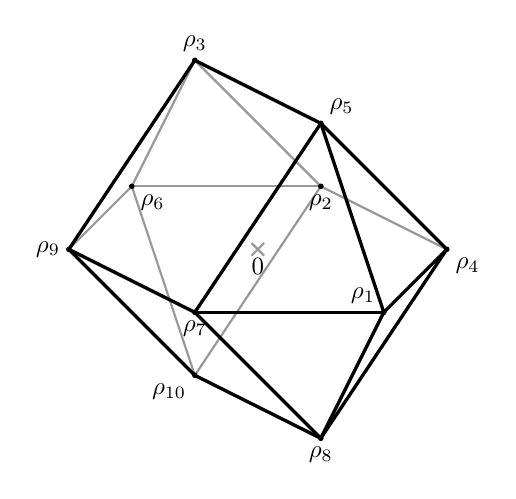
\begin{tikzpicture}[scale=0.8,every node/.style={scale=0.9}]
%background edges
\draw[gray!80, thick] (1,1) -- (-2,1);
\draw[gray!80, thick] (1,1) -- (-1,3);

\draw[gray!80, thick] (1,1) -- (3,0);
\draw[gray!80, thick] (-1,3) -- (-2,1);
\draw[gray!80, thick] (-3,0) -- (-2,1);
\draw[gray!80, thick] (1,1) -- (-1,-2);
\draw[gray!80, thick] (-1,-2) -- (-2,1);


%foreground edges
\draw[black, very thick] (-3,0) -- (-1,3);
\draw[black, very thick] (-3,0) -- (-1,-1);
\draw[black, very thick] (-1,-1) -- (1,2);
\draw[black, very thick] (1,2) -- (3,0);
\draw[black, very thick] (1,2) -- (2,-1);
\draw[black, very thick] (-1,-1) -- (2,-1);
\draw[black, very thick] (2,-1) -- (3,0);
\draw[black, very thick] (1,2) -- (-1,3);
\draw[black, very thick] (3,0) -- (1,-3);
\draw[black, very thick] (2,-1) -- (1,-3);
\draw[black, very thick] (-1,-2) -- (1,-3);
\draw[black, very thick] (-1,-2) -- (-3,0);
\draw[black, very thick] (-1,-1) -- (1,-3);

%origin 
\draw[gray!80, thick] (0.1,0.1) -- (-0.1,-0.1);
\draw[gray!80, thick] (-0.1,0.1) -- (0.1,-0.1);


%nodes
\filldraw[gray] (0,0) circle (0pt) node[anchor=north] {\textcolor{black}{$0$}};
\filldraw[black] (2,-1) circle (1pt) node[anchor=south east] {$\rho_1$};
\filldraw[black] (3,0) circle (1pt) node[anchor=north west] {$\rho_4$};
\filldraw[black] (1,1) circle (1pt) node[anchor=north] {$\rho_2$};
\filldraw[black] (-2,1) circle (1pt) node[anchor=north west] {$\rho_6$};
\filldraw[black] (-3,0) circle (1pt) node[anchor=east] {$\rho_9$};
\filldraw[black] (1,-3) circle (1pt) node[anchor=north] {$\rho_8$};
\filldraw[black] (-1,-2) circle (1pt) node[anchor=north east] {$\rho_{10}$};
\filldraw[black] (1,2) circle (1pt) node[anchor=south west] {$\rho_5$};
\filldraw[black] (-1,3) circle (1pt) node[anchor=south] {$\rho_3$};
\filldraw[black] (-1,-1) circle (1pt) node[anchor=north ] {$\rho_7$};



%\filldraw[black] (5,-3) circle (1pt) node[anchor=north west] {$(1,1,-1)$};
%\filldraw[gray] (2,-2) circle (1pt) node[label={[xshift=-0.9cm, yshift=-0.3cm]\textcolor{black}{$(0,1,-1)$}}]{};
%\filldraw[gray] (-6,-7) circle (1pt) node[label={[xshift=1.3cm, yshift=-0.3cm]\textcolor{black}{$(-1,-2,-2)$}}]{};
%\filldraw[black] (-2,-10) circle (1pt) node[anchor=north] {$(1,-3,-2)$};
%
%\filldraw[gray] (0,-3) circle (1pt) node[anchor=south east]{};
\end{tikzpicture}




		\caption{The polytope $P$ in Proposition~\ref{prop:definition_P_X}}
		\label{fig:P735}
	\end{figure}
	\begin{enumerate}
		\item $X$ is a K-polystable Fano $3$-fold with anticanonical volume $28$.
		\item The singular locus of $X$ consists of $4$ ordinary double points.
		\item The base of the  miniversal deformation of $X$ is smooth of dimension $4$, i.e.\ $\Def{X}$ is isomorphic to the formal spectrum of the power series ring $\CC \pow{t_\al, t_\beta, t_\gamma, t_\delta}$.
		\item $X$ deforms to the $2$nd entry in the Mori--Mukai list \cite{MM82,MM03} of smooth Fano $3$-folds with Picard rank $4$ (the other invariants are $(-K)^3 = 28$ and $h^{1,2} = 1$).
		\item The automorphism group $\Aut(P) \subset \mathrm{GL}(N) \simeq \mathrm{GL}_3(\ZZ)$ of the polytope $P$ is isomorphic to the semidirect product $D_8 \rtimes C_2$, where $C_2$ is the cyclic group of order $2$ and $D_8$ is the dihedral group of order $8$; more precisely, $\Aut(P)$ is generated by the following matrices:
		\begin{align*}
			g_1 &= \begin{pmatrix}
			-1 & 1 & 1 \\ 0 & 1 & 0 \\ 0 & 0 & 1
		\end{pmatrix}
		\text{ of order } 2, \\
			g_2 &= \begin{pmatrix}
			1 & 0 & 0 \\ 0 & 0 & 1 \\ 0 & 1 & 0
			\end{pmatrix}
		\text{ of order } 2, \\
			g_3 &= \begin{pmatrix}
			1 & -1 & 0 \\ 0 & 0 & 1 \\ 0 & -1 & 0
		\end{pmatrix}
		\text{ of order } 4.
		\end{align*}
		\item The automorphism group $\Aut(X)$ of $X$ is isomorphic to $T_N \rtimes \Aut(P)$, where $T_N = N \otimes_\ZZ \CC^*$ is the $3$-dimensional algebraic torus whose cocharacter lattice is $N$;
		\item the formal action of $\Aut(X)$ on $\Def{X} \simeq \Spf \CC \pow{t_\al, t_\beta, t_\gamma, t_\delta}$ is given by:
		\begin{enumerate}[label=$\bullet$]
			\item the torus $T_N$ acts linearly and diagonally on $t_\al, t_\beta, t_\gamma, t_\delta$ with weights $(0,1,1)$, $(0,1,-1)$, $(0,-1,-1)$ $(0,-1,1)$ in $M$, respectively,
			\item the involution $g_2$ leaves $t_\al$ and $t_\gamma$ fixed and swaps $t_\beta$ and $t_\delta$,
			\item the involution $g_1$ fixes everything,
			\item $g_3$ acts as $t_\al \mapsto - t_\beta$, $t_\beta \mapsto t_\gamma$, $t_\gamma \mapsto t_\delta$, $t_\delta \mapsto - t_\al$.
		\end{enumerate}
		\item The scheme $\Kps{3}{28}$ is smooth of dimension $2$ in a neighbourhood of the point $[X]$ corresponding to $X$. More precisely, $t_\al t_\beta t_\gamma t_\delta$ and $t_\al t_\gamma - t_\beta t_\delta$ are regular formal parameters of $\Kps{3}{28}$ at $[X]$.
		\item In a neighbourhood of $[X]$ in $\Kps{3}{28}$ the locus of non-smooth K-polystable Fano varieties is a smooth curve passing through $[X]$.
	\end{enumerate}
\end{prop}

The proof of (1--4) is contained in  \cite[\S5.1]{ask_petracci}; here we recap the argument briefly.


\begin{proof}
	The polytope $P$ has $20$ edges  (all of them have lattice length $1$) and has $12$ $2$-dimensional faces ($8$ of them are triangles and $4$ of them are quadrilaterals). It is depicted in Figure~\ref{fig:P735}.
	Let $\Sigma_X$ be the face fan of $P$.
	The $3$-dimensional cones of $\Sigma_X$ are
	\begin{equation}
		\begin{gathered}
			\sigma_{145}, \ \sigma_{157}, \ \sigma_{148}, \ \sigma_{178}, \\
			\sigma_{6910}, \ \sigma_{2610}, \ \sigma_{369}, \ \sigma_{236}, \\
			\sigma_{2345}, \ \sigma_{24810}, \
			\sigma_{78910}, \  \sigma_{3579}.
		\end{gathered}
	\end{equation}
Here $\sigma_{ijk}$ (resp.\ $\sigma_{ijkl}$) is the $3$-dimensional cone in $N$ whose rays are $\rho_i$, $\rho_j$, $\rho_k$ (resp.\ $\rho_i$, $\rho_j$, $\rho_k$, $\rho_l$).
	$X$ is the toric variety associated to $\Sigma_X$.
	
	\medskip
	
	(1) $X$ is Fano, because it is defined by the face fan of a Fano polytope.
	The polar $P^\circ$ of $P$ has normalised volume $28$, hence $(-K_X)^3 = 28$.
	Since $P = -P$ we have that the barycentre of $P^\circ$ is the origin, therefore $X$ is K-polystable by \cite[Corollary 1.2]{berman_polystability}.
	
	\medskip
	
	(2)	The simplicial cones of $\Sigma_X$ are smooth.
	The non-simplicial cones of $\Sigma_X$ are $\sigma_\al = \sigma_{2345}$, $\sigma_\beta = \sigma_{24810}$, $\sigma_\gamma = \sigma_{78910}$, $\sigma_\delta = \sigma_{3579}$.
	Let $U_\al$ (resp.\ $U_\beta$, $U_\gamma$, $U_\delta$) be the toric open affine subscheme of $X$  associated to the cone $\sigma_\al$ (resp.\ $\sigma_\beta$, $\sigma_\gamma$, $\sigma_\delta$), i.e.\ $U_\al = \Spec \CC[\sigma^\vee \cap M]$.
	
	Each of the cones $\sigma_\al$, $\sigma_\beta$, $\sigma_\gamma$, $\sigma_\delta$ is $\GL_3(\ZZ)$-equivalent to the cone over a unit square placed at height $1$, i.e.\ to the cone spanned by $e_3, e_1+e_3$, $e_2 + e_3$, $e_1 + e_2 + e_3$ in $\ZZ^3$ where $e_1, e_2, e_3$ is the standard basis of $\ZZ^3$.
	Therefore $U_\al$, $U_\beta$, $U_\gamma$, $U_\delta$ are all isomorphic to $\Spec \CC[x,y,z,w] / (xy-zw)$, which has an ordinary double point. Hence the singular locus of $X$ is made up of $4$ ordinary double points.
	
	More precisely, we fix an isomorphism between $U_\al$ (resp.\ $U_\beta$, $U_\gamma$, $U_\delta$)  and $\Spec \CC[x,y,z,w] / (xy-zw)$ by giving names to the minimal generators of the monoid $\sigma_\al^\vee \cap M$ (resp.\ $\sigma_\beta^\vee \cap M$, $\sigma_\gamma^\vee \cap M$, $\sigma_\delta^\vee \cap M$):
	\begin{equation*}
		\begin{gathered}
					x_\al = (-1,1,1) \quad y_\al = (1,0,0) \quad z_\al = (0,0,1) \quad w_\al = (0,1,0), \\
			x_\beta = (0,0,-1) \quad y_\beta = (0,1,0) \quad z_\beta = (-1,1,0) \quad w_\beta = (1,0,-1), \\
			x_\gamma = (0,-1,0) \quad y_\gamma = (0,0,-1) \quad z_\gamma = (-1,0,0) \quad w_\gamma = (1,-1,-1), \\
			x_\delta = (0,0,1) \quad y_\delta = (0,-1,0) \quad z_\delta = (-1,0,1) \quad w_\delta = (1,-1,0).
		\end{gathered}
	\end{equation*}

\medskip
	
	(3) Since $\rH^1(T_X) = 0$ and $\rH^2(T_X) = 0$ \cite[Lemma 4.4]{petracci_survey} and $X$ has isolated singularities, the deformations of $X$ can be identified with the deformations of the singularities of $X$ (see for instance \cite[\S14.2.1]{petracci_survey}).
	More precisely,  the product of the restriction maps
	\begin{equation} \label{eq:restriction_map_def_functors}
		\Def{X} \longrightarrow \Def{U_\al} \times \Def{U_\beta} \times \Def{U_\gamma} \times \Def{U_\delta}
	\end{equation}
 is smooth and induces an isomorphism on tangent spaces.
	Since an ordinary double point has a smooth $1$-dimensional miniversal deformation space, we conclude.
	
For future use we need to specify the meaning of $t_\al$, $t_\beta$, $t_\gamma$, $t_\delta$. We will always use the smooth functor
\begin{equation*}
	\Spf \CC \pow{t_\al} \longrightarrow \Def{U_\al},
\end{equation*}
	which induces an isomorphism on tangent spaces and is induced by the formal deformation of $U_\al$ over $\Spf \CC \pow{t_\al}$ given by the equation
\begin{equation} \label{eq:meaning_of_t_alpha}
	x_\al y_\al - z_\al w_\al + t_\al = 0,
\end{equation}
where the meaning of $x_\al$, $y_\al$, $z_\al$, $w_\al$ is specified in the proof of (2) above.
We make the similar conventions for $t_\beta$, $t_\gamma$ and $t_\delta$ and we will always stick to these conventions.
	
	\medskip
	
	(4) By \cite[Proposition~2.5]{ask_petracci} the $2$nd Betti number of $X$ is $4$. Since the smoothing of a $3$-fold ordinary double point has a Milnor fibre homotopically equivalent to the $3$-sphere, the $2$nd Betti number of the general smoothing of $X$ is $4$.
	Moreover, in smoothing $X$, also the anticanonical degree is preserved.
	In the Mori--Mukai list \cite{MM82, MM03} there is only one family of smooth Fano $3$-folds with Picard rank $4$ and anticanonical degree $28$.
	
	\medskip
	
	(5) We now compute the automorphism group of the polytope $P$. Any automorphism of $P$ should preserve the $\rho_1$-$\rho_6$ axis. There is only one reflection that switches $\rho_1$ and $\rho_6$, and we choose it as the generator of a $C_2$-subgroup of $\Aut(P)$. As a matrix in $\GL(N) = \GL_3(\ZZ)$ the generator of the $C_2$ above is 
	\[g_1=\begin{pmatrix}
	-1 & 1& 1 \\
 	0 & 1 & 0 \\
	0 & 0 & 1
	\end{pmatrix}.\]
All other automorphisms of $P$ fix $\rho_1$. They must also preserve the square obtained by intersecting $H$ with $P$, where $H = \RR \frac{\rho_2 + \rho_4}{2} + \RR \frac{\rho_3 + \rho_5}{2}$. This square has symmetry group $D_8$ and all of its symmetries lift uniquely to symmetries of $P$ that fix $\rho_1$. Moreover, these do not commute with the generator of $C_2$, thus $\Aut(P)= D_8 \rtimes C_2$. The matrix representations of the two generators of $D_8$ are:
	\[g_2=\begin{pmatrix}
	1 & 0& 0 \\
	0 & 0 & 1\\
	0 & 1 &0
	\end{pmatrix} \quad \text{ and } \quad
	g_3=\begin{pmatrix}
	1 & -1 & 0 \\
 	0 & 0 & 1 \\
	0 & -1 & 0
	\end{pmatrix}.
	\] 
	
	\medskip
	
	(6) This follows from \cite[Proposition~2.8]{ask_petracci} because no facet of the polar polytope $P^\circ$ has interior lattice points.
	
	\medskip
	
	(7) 	The vector space $\TT^1_X$, which is the tangent space of $\Def{X}$, is a $4$-dimensional representation of $\Aut(X) = T_N \rtimes \Aut(P)$.
	Using \eqref{eq:restriction_map_def_functors} we identify $\TT^1_X$ with the tangent space to the deformations of the $4$ singular points of $X$.
	
	The vector $(0,1,1) \in M$ is the only one such that by pairing with the primitive generators of the cone $\sigma_\al$, namely $\rho_2$, $\rho_3$, $\rho_4$, $\rho_5$, one gets $1$. In other words, $-(0,1,1) \in M$ is the vertex of $P^\circ$ which is dual to the face of $P$ whose vertices are $\rho_2$, $\rho_3$, $\rho_4$, $\rho_5$.
	By \cite{altmann_t1} $\TT^1_{U_\al}$ is the $1$-dimensional representation of the torus $T_N = N \otimes_\ZZ \CC^*$ with weight $(0,-1,-1)$. This implies that the coordinate $t_\al$ has degree $(0,1,1) \in M$ with respect to $T_N$.
	
	In similar ways one proves that $t_\beta$, $t_\gamma$, $t_\delta$ have degrees $(0,-1,1)$, $(0,1,1)$, $(0,1,-1)$ respectively. We now focus on the action of the $3$ generators $g_1$, $g_2$, $g_3$ of $\pi_0(\Aut(X))$ given in (5).
	
	\smallskip
	
	The involution $g_1$ acts on the vertices of $P$ by $\rho_i \leftrightarrow \rho_{i+5}$ for each $i \in \{1,\dots,5\}$. In particular, by remembering that the torus orbits on $X$ correspond bijectively to the cones of the face fan of $P$, we can see that $U_\al$ is $g_1$-invariant and $g_1$ acts via pull-back on the regular functions of $U_\al$. For example
	\[
	g_1(x_\al) = \begin{pmatrix}
		-1 & 1 & 1
	\end{pmatrix}
\begin{pmatrix}
	-1 & 1 & 1 \\
	0 & 0 & 1 \\
	0 & 1 & 0
\end{pmatrix}
=
\begin{pmatrix}
	1 & 0 & 0
\end{pmatrix}
= y_\al
	\]
	and
		\[
	g_1(z_\al) = \begin{pmatrix}
		0 & 0 & 1
	\end{pmatrix}
	\begin{pmatrix}
		-1 & 1 & 1 \\
		0 & 0 & 1 \\
		0 & 1 & 0
	\end{pmatrix}
	=
	\begin{pmatrix}
		0 & 1 & 0
	\end{pmatrix}
	= w_\al.
	\]
	This shows that $g_1$ maps the miniversal deformation \eqref{eq:meaning_of_t_alpha} of $U_\al$ to itself. Hence $g_1$ maps $t_\al$ to itself.
	In a similar way, one can show that $U_\beta$, $U_\gamma$ and $U_\delta$ are $g_1$-invariant and $g_1$ fixes $t_\beta$, $t_\gamma$ and $t_\delta$ too.
	
	\smallskip
	
	Let us now focus on $g_2$. On the vertices of $P$ this involution acts as $\rho_2 \leftrightarrow \rho_3$, $\rho_4 \leftrightarrow \rho_5$, $\rho_7 \leftrightarrow \rho_8$, $\rho_9 \leftrightarrow \rho_{10}$ and fixes $\rho_1$ and $\rho_6$.
	One can see that $U_\al$ is $g_2$-invariant and $g_2(x_\al) = x_\al$, $g_2(y_\al) = y_\al$, $g_2(z_\al) = w_\al$. Therefore $g_2$ maps the miniversal deformation \eqref{eq:meaning_of_t_alpha} of $U_\al$ to itself, hence $t_\al$ is fixed by $g_2$.
	
	One sees that $g_2(U_\beta) = U_\delta$. So, via pull-back, $g_2$ maps a regular function on $U_\delta$ to a regular function on $U_\beta$.
	A similar calculation as above gives $g_2(y_\delta)=x_\beta$, $g_2(x_\delta) = y_\beta$, $g_2(z_\delta) = z_\beta$, $g_2(w_\delta) = w_\beta$.
	So the miniversal deformation $x_\delta y_\delta - z_\delta w_\delta + t_\delta = 0$ of $U_\delta$ is mapped by $g_2$ to 
	the deformation $x_\beta y_\beta - z_\beta w_\beta + t_\delta = 0$ of $U_\beta$. This latter deformation is induced by the chosen miniversal deformation $x_\beta y_\beta - z_\beta w_\beta + t_\beta = 0$ of $U_\beta$ by setting $t_\delta = t_\beta$. Therefore $g_2$ swaps $t_\delta$ and $t_\beta$.
	
	In a similar way, one can show that $g_2$ leaves $t_\gamma$ fixed.
	
	
	\smallskip
	
	Let us now focus on $g_3$.
	The order $4$ matrix $g_3$ acts as follows on the vertices of $P$: $\rho_1$ and $\rho_6$ are fixed and there are two orbits of cardinality $4$, namely $\rho_2 \mapsto \rho_{10} \mapsto \rho_9 \mapsto \rho_3 \mapsto \rho_2$ and $\rho_5 \mapsto \rho_4 \mapsto \rho_8 \mapsto \rho_7 \mapsto \rho_5$.
	
	One sees $g_3(U_\al) = U_\beta$.
	Via pull-back along $g_3$, we get $x_\beta \mapsto w_\al$, $y_\beta \mapsto z_\al$, $z_\beta \mapsto x_\al$, $w_\beta \mapsto y_\al$.
	So the miniversal deformation $x_\beta y_\beta - z_\beta w_\beta + t_\beta = 0$ of $U_\beta$ is mapped via $g_3$ to the deformation $w_\al z_\al - x_\al y_\al + t_\beta = 0$ of $U_\al$.
	This shows that $g_3$ maps $t_\al$ to $- t_\beta$.
	
	In a similar way, one obtains $g_3(U_\beta) = U_\gamma$, $g_3(U_\gamma) = U_\delta$, $g_3(U_\delta) = U_\al$ and that $g_3$ acts as $t_\beta \mapsto t_\gamma \mapsto t_\delta \mapsto - t_\al$.
	
	
	
	
	
	
	\medskip
	
	(8) By (7) the invariant subring of the formal action of the torus $T_N \simeq (\CC^*)^3$ on $\CC \pow{t_\al, t_\beta, t_\gamma, t_\delta}$ is  $\CC \pow{t_\al t_\gamma, t_\beta t_\delta}$, which is a power series ring in $2$ indeterminates.
	The involutions $g_1$ and $g_2$ act trivially on $\CC \pow{t_\al t_\gamma, t_\beta t_\delta}$, whereas $g_3$ acts on $\CC \pow{t_\al t_\gamma, t_\beta t_\delta}$ with order $2$ and maps $t_\al t_\gamma$ to $- t_\beta t_\delta$.
	In conclusion, the subring of $\CC \pow{t_\al, t_\beta, t_\gamma, t_\delta}$ of the invariants elements under the action of $\Aut(X)$ is $\CC \pow{t_\al t_\beta t_\gamma t_\delta, t_\al t_\gamma - t_\beta t_\delta}$, which is a power series ring in $2$ indeterminates.
	
	By the Luna  \'etale slice theorem for algebraic stacks \cite{luna_etale_slice_stacks} the local structure of $\Kss{3}{28} \to \Kps{3}{28}$ at the point $[X]$ is given by the  commutative square
	\begin{equation*}
		\xymatrix{
			\left[ \Spf \CC \pow{t_\al, t_\beta, t_\gamma, t_\delta} \ / \ \Aut(X)  \right] \ar[d] \ar[r] & \Kss{3}{28}  \ar[d] \\
			\Spf \CC \pow{t_\al t_\beta t_\gamma t_\delta, t_\al t_\gamma - t_\beta t_\delta} \ar[r] &  \Kps{3}{28}
		}
	\end{equation*}
	where the horizontal maps are formally \'etale and maps the closed point to $[X]$.
	This implies that $\Kps{3}{28}$ is smooth of dimension $2$ near $[X]$ and that $t_\al t_\beta t_\gamma t_\delta$, $t_\al t_\gamma - t_\beta t_\delta$ are local analytic coordinates.

	
	\medskip
	
	(9) Here, to simplify, we work in the analytic category.
	Since $t_\al, t_\beta, t_\gamma, t_\delta$ are the smoothing parameters of an ordinary double point, it is clear that in the miniversal deformation of $X$, which now we think over a small polydisc $\Delta^4$ of dimension $4$ (with local analytic coordinates $t_\al, t_\beta, t_\gamma, t_\delta$), the smooth fibres are exactly those where $t_\al \neq 0$, $t_\beta \neq 0$, $t_\gamma \neq 0$, $t_\delta \neq 0$.
	Let $D$ be the discriminant locus, i.e.\ the locus in the base space $\Delta^4$ of the miniversal deformation of $X$ where the fibres are singular; hence $D = \{ t_\al t_\beta t_\gamma t_\delta = 0  \} \subset \Delta^4$ is the union of $4$ hyperplanes.
	
	Let $\Delta^2$ be a small $2$-dimensional polydisc which gives the local structure of $\Kps{3}{28}$ at $[X]$.
	The holomorphic map $\Delta^4 \to \Delta^2$ is given by
	\[
	(t_\al, t_\beta, t_\gamma, t_\delta) \mapsto (t_\al t_\beta t_\gamma t_\delta, t_\al t_\gamma - t_\beta t_\delta).
	\]
	The image of $D$ via this map is clearly a germ of a smooth curve passing through the origin.
	The image of $D$ is exactly the locus in $\Delta^2$ of singular K-polystable Fanos close to $[X]$.
\end{proof}

An immediate consequence of Proposition~\ref{prop:definition_P_X} is:

\begin{cor} \label{cor:almost_everything_without_rationality}
	Let $M := \Kps{3}{28}$ the K-moduli space of K-polystable Fano $3$-folds with anticanonical volume $28$.
	Let $\modulismooth \subset M$ be the locus which parametrises the smooth K-polystable Fano $3$-folds with anticanonical volume $28$ and Picard rank $4$.
	Then there exists an open subscheme $U$ of $M$ such that $U$ is a smooth surface and $U \setminus \modulismooth$ is a smooth curve.
\end{cor}

This is a portion of Theorem~\ref{thm:main}; the only things which are missing are the statements about the rationality of $U$ and of $U \setminus \modulismooth$.


\section{Embeddings in toric varieties}

Now we realise the toric Fano $3$-fold $X$ of Proposition~\ref{prop:definition_P_X} inside a toric Fano $4$-fold.

\begin{prop} \label{prop:X_inside_F}
	In the lattice $N_F = \ZZ^4$ consider the lattice polytope $P_F$ whose vertices are the columns $r_1, \dots, r_7 \in N_F$ of the matrix
	\[
	R_F=
	\begin{bmatrix}
		1 & 0 & -1 & 0 & 0 & 0 & 0 \\
		0 & 1 & 0 & -1 & 0 & 0 & 0 \\
		0 & 0 & -1 & -1 & 1 & -1 & 0 \\
		0 & 0 & -1 & -1 & 0 & -1 & 1
	\end{bmatrix}.
	\]
	Let $F$ be the toric variety associated to the face fan of $P_F$.
	Then:
	\begin{enumerate}
		\item $F$ is a smooth Fano $4$-fold and is the GIT quotient $\AA^7 \git (\CC^*)^3$ given by the weight matrix 
		\[\begin{matrix}
			u_1& u_2& u_3& u_4&u_5&u_6&u_7\\
			\hline 
1 & 0 & 1 & 0 & 0 & -1 & 0 \\
0 & 1 & 0 & 1 & 0 & -1 & 0 \\
0 & 0 & 0 & 0 & 1 & 1 & 1
		\end{matrix}\]
	and by the stability condition $(1,1,1)$;
	\item if $X$ is the toric Fano $3$-fold considered in Proposition~\ref{prop:definition_P_X}, then the linear map $N_X = \ZZ^3 \to N_F = \ZZ^4$ induced by the matrix
	\[
	A = \begin{bmatrix}
		0 & 1 & 0 \\
		0 & 0 & 1 \\
		-1 & 1 & 1 \\
		1 & 0 & 0
	\end{bmatrix}
	\]
induces a toric morphism $X \to F$ which is a closed embedding and identifies $X$ with the divisor in $F$ defined by the equation
\begin{equation*}
u_5 u_7 - u_6^2 u_1 u_2 u_3 u_4 = 0
\end{equation*}
in the Cox coordinates of $F$.
	\end{enumerate}
\end{prop}	
%
\begin{remark}
The weight matrix of $F$ and the line bundle $L=~\mathcal{O}_Y\begin{pmatrix}0\\0\\2\end{pmatrix}$ of which the equation of $X$ is a section of have previously appeared in \cite{quantum_periods}[\S 87]. We refer to the analysis there justifying why the Picard rank of $X$ is $4$, whereas the Picard rank of its ambient space $F$ is $3$.
\end{remark}

\begin{proof}
(1) The divisor sequence \cite{cox_little_schenck}[Theorem 4.1.3] of $F$ is
\begin{equation*}
	0 \longrightarrow M_F \simeq \ZZ^4 \xrightarrow{(R_F)^T}  \Div_T(F) \simeq \ZZ^7 \overset{D_F}{\longrightarrow}  \Pic(F) \simeq \ZZ^3 \longrightarrow 0
\end{equation*}
%\begin{equation*}
%	0 \longrightarrow \ZZ^3 \xrightarrow{(D_F)^T} \Div_T(F)^\vee \xrightarrow{R_F} N_F \longrightarrow 0
%\end{equation*}
where $D_F$ is the $3 \times 7$ matrix in the statement (1).

Thus $D_F$ is the weight matrix for $F$; in other words, the action of the torus $(\CC^*)^3$ on $\AA^7$ with weights given by $D_F$ is such that the corresponding GIT quotient $\AA^7 \git (\CC^*)^3$ with respect to a certain stability condition.
Since $F$ is Fano and $-K_F$ is the $(\CC^*)^3$-linearised line bundle on the quotient with weights $(1,1,3) \in \Pic(F) \simeq \ZZ^3$, the stability condition is given by the chamber which contains $(1,1,3)$. This chamber also contains $(1,1,1)$, as it is the positive orthant.

 It is immediate to check that $F$ is smooth as all relevant $3 \times 3$ minors of $R_F$ are equal to $\pm1$.

\medskip

(2) Let $\rho_1, \dots, \rho_{10}$ be the vectors in \eqref{eq:rays_of_X}, i.e.\ the primitive generators of the rays of the fan defining $X$. 
The map induced by $A$ sends the $\rho_i$'s onto the plane with normal vector $m_X:=(1,1,-1,-1)$: 
\[ A 
\left(\begin{array}{c|c|c}
\rho_1 & \cdots & \rho_{10}
\end{array}\right)
= \begin{bmatrix}
		0 & 1 &0 &1 &0 &0 &-1& 0 &-1& 0  \\
		0 &0 &1 &0 &1 &0 &0 &-1& 0& -1\\
		-1 &1& 1& 0& 0& 1& -1& -1& 0& 0\\
		1& 0& 0& 1& 1& -1& 0 &0 &-1 &-1
	\end{bmatrix}.
	\]
One can check that each cone of $\Sigma_X$ is sent via $A$ to a cone in $\Sigma_F$. Furthermore, the image of the fan $\Sigma_X$ equals the intersection of the hyperplane $m_X^\perp$ with $\Sigma_F$.
Therefore the image of the toric morphism $X \to F$ is a prime divisor on $F$. We want to determine its equation in the Cox coordinates of $F$.


Each lattice element $A(\rho_i)$ belongs to exactly one 2-dimensional cone of $F$.
Let us write it as a linear combination, with positive coefficients, of the the primitive generators of the fan $\Sigma_F$. For instance
\[
A(\rho_1)=(0,0,-1,1)^T=(0,0,-1,-1)^T+2(0,0,0,1)^T=r_6+2r_7.
\]
The matrix which express these combinations is
\[
\begin{array}{c|ccccccc}
	& r_1 &r_2&r_3&r_4 &r_5& r_6 &r_7  \\
	\hline   A(\rho_1) &  0 &0 &0 &0 &0 &1 &2   \\
	A(\rho_2) & 	1& 0 &0& 0& 1& 0& 0 \\
	A(\rho_3) & 	0 &1& 0 &0 &1 &0 &0  \\
	A(\rho_4) & 	1 &0 &0 &0 &0& 0& 1 \\
	A(\rho_5) &     0 &1 &0& 0& 0& 0& 1 \\
	A(\rho_6) &     0 &0 &0& 0& 2& 1& 0 \\
	A(\rho_7) &     0 &0 &1& 0& 0& 0& 1\\ 
	A(\rho_8) &     0 &0 &0& 1& 0& 0& 1\\ 
	A(\rho_9) &     0 &0 &1& 0& 1& 0& 0\\ 
	A(\rho_{10}) &  0 &0 &0& 1& 1& 0& 0\\ 
\end{array}
\]
Let $B$ be the $7 \times 10$ matrix given by transposing this matrix.
We have a commutative diagram with exact rows
\begin{equation*}
	\begin{aligned}
		\xymatrix{
			&&&&& \ZZ  \\
			0  \ar[r] & (\Pic(F))^\vee \ar[rr] &&(\Div_T F)^\vee  \ar[rr]^{R_F} &&N_F\ar@{->>}[u]^{m_X}\ar[r] &0 \\
			0  \ar[r]& (\Cl(X))^\vee \ar[u] \ar[rr]&& (\Div_T X)^\vee \ar[u]^{B^T}  \ar[rr]^{R_X} &&N_X\ar[u]^{A}\ar[r] &0 \\
		}
	\end{aligned}
\end{equation*}
which dualises to
\begin{equation*}
	\begin{aligned}
		\xymatrix{ & \ZZ \ar[d]^{m_X} \\
			0  \ar[r] & M_F \ar[d]^{A^T} \ar[rr]^{R_F^T} && \Div_T F  \ar[rr]^{D_F} \ar[d]^B &&\Pic(F) \ar[d] \ar[r] &0 \\
			0  \ar[r]& M_X \ar[rr]^{R_X^T} &&  \Div_T X   \ar[rr]^{R_X} && \Cl(X) \ar[r] &0 
		}
	\end{aligned}
\end{equation*}
where the two exact rows are the divisor sequences. The map $B \colon \Div_T F \to \Div_T X$ is the pull-back of torus-invariant divisors on $F$ along the morphism $X \to F$. In terms of Cox coordinates we have the following.
\begin{align*}
	%\CC[u_1,\ldots, u_7]& \to \CC[x_1,\ldots, x_{10}] \\
u_1& \mapsto x_2x_4\\
u_2& \mapsto x_3x_5\\
u_3& \mapsto x_7x_9\\
u_4& \mapsto x_8x_{10}\\
u_5& \mapsto x_2x_3x_6^2x_9x_{10}\\
u_6& \mapsto x_1x_6\\
u_7& \mapsto x_1^2x_4x_5x_7x_8
\end{align*}
It is clear that the equation describing the image of $X$ in $F$ is
\[
u_5u_7=u_6^2u_1u_2u_3u_4.
\]

It remains to check that the toric morphism $X \to F$ is a closed embedding. This can be checked locally by analysing the affine charts.
\end{proof}

\begin{comment}
\begin{proof} (Alternative proof)
The map $N_X\hookrightarrow N_F$ induces an injection of tori \[T_X\simeq (\CC^*)^3\mapsto T_F\simeq (\CC^*)^4_{t_1,\ldots,t_4}\] whose image has the equation $t_1t_2=t_3t_4$. Since $T_F\stackrel{R_F}{\simeq}(\CC^*)^7_{s_1,\ldots,s_7}/(\CC^*)^3$ we substitute and obtain \begin{align*}s_1s_3^{-1}s_2s_4^{-1}&=s_3^{-1}s_4^{-1}s_5s_6^{-1}s_3^{-1}s_4^{-1}s_6^{-1}s_7\\
\Leftrightarrow s_6^2s_1s_2s_3s_4&=s_7s_5,
\end{align*} which we compactify to obtain the corresponding equation in the Cox coordinates $u_i$ on $F$. \end{proof}
\end{comment}


\section{Deforming a toric variety}

In Proposition~\ref{prop:X_inside_F} we have seen that the toric Fano $3$-fold $X$ of Proposition~\ref{prop:definition_P_X} is a divisor inside a smooth toric Fano $4$-fold $F$.
Now we show that a particular $4$-dimensional subspace of the linear system $\vert \cO_F(X) \vert$ gives the miniversal ($\QQ$-Gorenstein) deformation of $X$.


\begin{prop} \label{prop:deforming_X_inside_F}
	Let $X$ be the toric Fano $3$-fold in Proposition~\ref{prop:definition_P_X}
	and let $F$ be the toric Fano $4$-fold in Proposition~\ref{prop:deforming_X_inside_F}.
	Let $u_1, \dots, u_7$ denote the Cox coordinates of $F$ as in Proposition~\ref{prop:X_inside_F}.
	Consider the $4$-parameter flat family
	\[
	\cX \to \AA^4 = \Spec \CC [c_1, c_2, c_3, c_4]
	\]
	 given by the equation
	 \begin{equation} \label{eq:equation_of_X_inside_F}
	 		u_5u_7-u_1u_2u_3u_4u_6^2+u_6^2(c_1u_1^2u_2^2+c_2 u_1^2u_4^2+ c_3 u_2^2u_3^2+c_4 u_3^2u_4^2)=0
	 \end{equation}
	inside $F$.
	
	Then the base change of $\cX \to \AA^4$ to $\Spf \CC \pow{c_1, c_2, c_3, c_4}$ is the miniversal ($\QQ$-Gorenstein) deformation of $X$.
	Moreover, the discriminant locus (i.e.\ the locus in $\AA^4$ where the fibres of $\cX \to \AA^4$ are singular) and the divisor $\{ c_1 c_2 c_3 c_4 = 0  \} \subset \AA^4$ coincide in a neighbourhood of the origin in $\AA^4$.
\end{prop}

We put the word $\QQ$-Gorenstein in parenthesis because the miniversal deformation of $X$ coincides with the miniversal $\QQ$-Gorenstein deformation of $X$, since every infinitesimal deformation of $X$ is automatically $\QQ$-Gorenstein because $X$ is Gorenstein.


The fact that the fibre of $\cX \to \AA^4$ over the origin is exactly $X$ is the content of Proposition~\ref{prop:deforming_X_inside_F}. Hence we need to prove the versality of this deformation.
Before doing this we prove some preliminary lemmata.









\begin{lemma} \label{lemma:sequence_of_polynomials}
Let $s_1, s_2, s_3, x, y$ be indeterminates. Consider the polynomial ring $R = \CC[s_1, s_2, s_3, x, y]$ with $\NN$-grading given by $\deg s_1 = \deg s_2 = \deg s_3 = 1$ and $\deg x = \deg y = 0$.
 For every $k \in \NN$,
 \begin{itemize}
 	\item  let $R_k$ be the homogenous summand of $R$ of degree $k$, i.e.\ the $\CC$-vector subspace of $R$ with basis
 	\[
 	\left\{ s_1^{i_1} s_2^{i_2} s_3^{i_3} x^m y^n \mid i_1, i_2, i_3, m,n \in \NN, \ i_1 + i_2 + i_3 = k  \right\};
 	\]
 	\item set $R_{\leq k} = \bigoplus_{0\leq i \leq k} R_i$, which is the $\CC$-vector subspace of $R$ with basis
 	\[
 	\left\{ s_1^{i_1} s_2^{i_2} s_3^{i_3} x^m y^n \mid i_1, i_2, i_3, m,n \in \NN, \ i_1 + i_2 + i_3 \leq k  \right\};
 	\]
 	\item set $R_{\geq k} = \bigoplus_{ i \geq k} R_i$, which is the ideal $(s_1,s_2,s_3)^k$ of $R$.
 \end{itemize}

Then there exist two sequences $\{  x_k \}_{k \in \NN}$ and $\{  y_k \}_{k \in \NN}$ of polynomials such that:
\begin{enumerate}
	\item $x_0 = x$ and $y_0 = y$,
	\item for every $k \in \NN^+$, $x_k \in R_{\leq k} \cap (x,y)$ and $y_k \in R_{\leq k} \cap (x,y)$,

	\item for every $k \in \NN^+$, $x_k - x_{k-1} \in R_{k}$ and $y_k - y_{k-1} \in R_{k}$,
	
	\item for every $k \in \NN^+$, $f_k := x_k y_k - (xy + s_1 x^2 + s_2 y^2 + s_3 x^2 y^2)$ lies in the ideal $R_{\geq k+1} \cap (x,y)^2$.

\end{enumerate}
\end{lemma}

By (3) the sequences of the $x_k$'s and of the $y_k$'s give two elements of the ring  $\CC[x,y] \pow{s_1, s_2, s_3}$. By (4) the product of these two power series is $xy + s_1 x^2 +s_2 y^2 + s_3 x^2 y^2$.

\begin{proof}[Proof of Lemma~\ref{lemma:sequence_of_polynomials}]
	We proceed by induction on $k \in \NN^+$. In the base case $k=1$ we take $x_1 = x - s_2 y + s_3 x^2 y$ and $y_1 = y + s_1 x$. Obviously (2) and (3) hold. Moreover,
	\[
	f_1 = x_1 y_1 - (xy + s_1 x^2 + s_2 y^2 + s_3 x^2 y^2) = s_1 s_2 xy + s_1 s_3 x^3 y
	\]
	lies in $(s_1, s_2, s_3)^2 \cap (x,y)^2$; this gives (4).
	
	Now we do the inductive step. Fix $k \in \NN^+$ and assume that we have $x_0, \dots, x_k$ and $y_0, \dots, y_k$ which satisfy (2)-(4);  we shall construct $x_{k+1}$ and $y_{k+1}$.
	
By (4) $f_k \in (x,y)^2 \subset (x,y)$, so there exist polynomials $A$ and $B$ such that $f_k = Ax + By$.
We can assume that there are no cancellations between $Ax$ and $By$, for instance by requiring that $B \in \CC[s_1, s_2, s_3, y]$.
Since by (3) $f_k \in R_{\geq k+1}$, we have  $A, B \in R_{\geq k+1}$.
Let $a$ (resp.\ $b$) the homogeneous part of $A$ (resp.\ $B$) of degree $k+1$. So $a, b \in R_{k+1}$ and $A-a, B-b \in R_{\geq k+2}$.
Moreover, since $f_k \in (x,y)^2$ we have $A, B \in (x,y)$, and consequently $a,b \in (x,y)$.

Set
\begin{equation*}
	x_{k+1} = x_k - b \quad \text{and} \quad y_{k+1} = y_k - a.
\end{equation*}
By the inductive hypothesis we have $x_k, y_k \in R_{\leq k} \cap (x,y)$ and by construction we have $a,b \in R_{k+1} \cap (x,y)$; therefore $x_{k+1}$ and $y_{k+1}$ lie in $R_{\leq k+1} \cap (x,y)$; this is (2) for $k+1$.
Clearly we also have (3) for $k+1$.

We have
\begin{align*}
	f_{k+1} &= x_{k+1} y_{k+1} - (xy + s_1 x^2 + s_2 y^2 + s_3 x^2 y^2) \\
	&= (x_k - b)(y_k - a) - (xy + s_1 x^2 + s_2 y^2 + s_3 x^2 y^2) \\
	&= f_k -b y_k - a x_k +ab \\
	&= (Ax + By) - a x_k - b y_k +ab.
\end{align*}
Since $A,B,a,b,x_k,y_k \in (x,y)$ we get $f_{k+1} \in (x,y)^2$.
Moreover, we can write
\[
f_{k+1} = a(x-x_k) + (A-a) x + b(y-y_k) + (B-b) y + ab.
\]
Since $a,b \in R_{k+1}$, $A-a, B-b \in R_{\geq k+2}$ and $x-x_k, y-y_k \in R_{\geq 1}$, we have $f_{k+1} \in R_{\geq k+2}$. We have obtained (4) for $k+1$.
\end{proof}




\begin{lemma} \label{lemma:two_deformations_are_isomorphic}
Consider the affine $3$-fold $U = \Spec \CC [ x,y,z,w]  / (xy-zw)$.
Then the two formal deformations of $U$ over $\Spf \CC \pow{s_1, s_2, s_3, s_4}$ given by
\[
xy-zw + s_1 x^2 + s_2 y^2 + s_3 x^2 y^2 + s_4 = 0
\]
and by
\[
xy-zw + s_4 =0,
\]
respectively,
are isomorphic.
\end{lemma}

\begin{proof}
Fix $k \in \NN$. Consider the finite $\CC$-algebra
\[
S_k = \CC[s_1, s_2, s_3, s_4]/(s_1, s_2, s_3, s_4)^{k+1}
\]
 and the following two $S_k$-algebras
\begin{align*}
		A_k &= S_k[x,y,z,w] / (xy-zw + s_4), \\
	B_k &= S_k[x,y,z,w] / (xy-zw + s_1 x^2 + s_2 y^2 + s_3 x^2 y^2 + s_4).
\end{align*}
Let $x_k$ and $y_k$ be the polynomials constructed in Lemma~\ref{lemma:sequence_of_polynomials}.
By (4) one can
consider the $S_k$-algebra homomorphism $\phi_k \colon A_k \to B_k$ given by $x \mapsto x_k$, $y \mapsto y_k$, $z \mapsto z$, $w \mapsto w$.
By (1) and (2) we have $x - x_k \in (s_1, s_2, s_3, s_4)$, so $\phi_k$ is just a translation, hence it is invertible.

By (3) we have
\[
x_k \equiv x_{k-1} \mod (s_1, s_2, s_3, s_4)^k \quad \text{and} \quad y_k \equiv y_{k-1} \mod (s_1, s_2, s_3, s_4)^k.
\]
So $\phi_k$ and $\phi_{k-1}$ are equal modulo $(s_1, s_2, s_3, s_4)^k$. More precisely, by using the natural projection $S_k \onto S_{k-1}$ we get that $\phi_k \otimes_{S_k} \mathrm{id}_{S_{k-1}}$ and $\phi_{k-1}$ are equal as isomorphisms from $A_{k-1} = A_k \otimes_{S_k} S_{k-1}$ to $B_{k-1} = B_k \otimes_{S_k} S_{k-1}$.
Therefore the system of isomorphisms $\phi_k$'s gives the required isomorphism of formal deformations of $U$.
\end{proof}

\begin{comment}
\begin{prop}
\textcolor{blue}{rewrite this in general, with x,y,z,w instead of $u_i$}
There exists an automorphism \begin{align*}\CC\pow{c_1,\ldots,c_4}[u_1,u_2,u_5, u_7] &\to \CC\pow{c_1,\ldots,c_4}[u_1,u_2,u_5, u_7]\\
c_i&\mapsto c_i,  \, i\in \{1,\ldots,4\}\\
u_1&\mapsto \overline{u_1},  \ \ u_5\mapsto u_5\\
u_2&\mapsto \overline{u_2},  \ \ u_7\mapsto u_7\\
\end{align*}
where $\overline{u_1}\cdot\overline{u_2}=  u_1u_2+c_1u_1^2u_2^2 + c_2 u_1^2+ c_3u_2^2$. This induces a ring homomorphism $\CC \pow{t_\alpha} \to \CC \pow{c_1,\ldots,c_4}$ taking $t_\al \to c_4$ \textcolor{blue}{[conclusion?]}.
\end{prop}
 
 \begin{proof}
We prove the claim by induction. Let $\overline{u_1}, \overline{u_2}\in R_k=\dfrac{\CC[u_1,u_2,c_1,c_2,c_3]}{(c_1,c_2,c_3)^k}$ such that $\overline{u_1}\cdot\overline{u_2}=  u_1u_2+c_1u_1^2u_2^2 + c_2 u_1^2+ c_3u_2^2$. We can assume that both $\overline{u_1}$ and $\overline{u_2}$ contain no pure monomials in the $c_i$. We show that there exist $\overline{\overline{u_1}}, \overline{\overline{u_2}}\in R_{k+1}$ such that  \[\overline{\overline{u_1}}\cdot  \overline{\overline{u_2}} =u_1u_2+c_1u_1^2u_2^2 + c_2 u_1^2+ c_3u_2^2\textup{ in }R_{k+1}\] and moreover 
$\overline{u_i}$ is the image of $\overline{\overline{u_1}}$ via the natural map $R_{k+1}\to R_{k}$.

For $k=1$, choose $\overline{u_1}=u_1$ and $\overline{u_2}=u_2$. For $k=2$, choose $\overline{u_1}=u_1-c_2u_2-c_1u_1^2u_2$ and $\overline{u_2}=u_2-c_3u_1$.

For $k>2$, since $R_k\subset R_{k+1}$ we may abuse notation and consider \[f=\overline{u_1}\cdot\overline{u_2} - (u_1u_2 +c_1u_1^2u_2^2 + c_2 u_1^2+ c_3u_2^2)\in R_{k+1}.\]
The induction hypothesis implies that $f$ contains no pure monomials in the $c_i$. We can therefore split $f=Au_1+Bu_2$ where $A, B\in (c_1,c_2,c_3)^{k+1}\setminus (c_1,c_2,c_3)^{k+2}$ and now choose $\overline{\overline{u_1}}=\overline{u_1}-B$ and $\overline{\overline{u_2}}=\overline{u_2}-A$. We then have
\begin{align*}
\overline{\overline{u_1}}\cdot \overline{\overline{u_2}}=&\overline{u_1}\cdot \overline{u_2}-\overline{u_1}A+AB-\overline{u_2}B\\
=&f+u_1u_2 +c_1u_1^2u_2^2 + c_2 u_1^2+ c_3u_2^2-\overline{u_1}A+AB-\overline{u_2}B\\
=&u_1u_2 +c_1u_1^2u_2^2 + c_2 u_1^2+ c_3u_2^2 + A(u_1-\overline{u_1})+B(u_2-\overline{u_2})+AB.
\end{align*}
Since $A(u_1-\overline{u_1})$, $B(u_2-\overline{u_2})$ and $AB$ are all in $(c_1,c_2,c_3)^{k+2}$, we are able to conclude.

\end{proof}
\end{comment}




\begin{lemma}\label{lemma:discriminant_locus_def_3ODP}
Consider the affine $3$-fold $U = \Spec \CC [ x,y,z,w]  / (xy-zw)$ and consider the flat deformation $\cU \to \AA^4 = \Spec \CC [s_1, s_2, s_3, s_4]$ of $U$ given by the equation
\begin{equation} \label{eq:deformed}
xy-zw + s_1 x^2 + s_2 y^2 + s_3 x^2 y^2 + s_4 = 0.
\end{equation}

Then the discriminant locus of $\cU \to \AA^4$, i.e.\ the locus in $\AA^4$ over which the fibres of $\cU \to \AA^4$ are singular, is the vanishing locus of
\begin{equation} \label{eq:discriminant}
s_4 (16 s_1^2 s_2^2 - 32 s_1 s_2 s_3 s_4 - 8 s_1 s_2 + 16 s_3^2 s_4^2 - 8 s_3 s_4 + 1).
\end{equation}
In particular, in a neighbourhood of $0$ in $\AA^4$ the discriminant locus coincides with the hyperplane $\{s_4 = 0\}$.
\end{lemma}



\begin{proof}
	Let $f \in \CC[s_1, s_2, s_3, s_4, x, y, z, w]$ be the polynomial appearing in \eqref{eq:deformed}.
	Consider the ideal $J \subseteq \CC[s_1, s_2, s_3, s_4, x, y, z, w]$ generated by $f$ and by the $4$ partial derivatives of $f$ with respect to $x$, $y$, $z$  and $w$.
	By the Jacobian criterion and \cite[\S3.2]{cox_little_oshea}, the discriminant locus in $\AA^4 = \Spec \CC [s_1,s_2,s_3,s_4]$ is defined by the ideal $J \cap \CC[s_1, s_2, s_3, s_4]$. By \cite[Theorem~3.1.2]{cox_little_oshea} this last ideal can be easily computed with any computer algebra software by taking a Gr\"obner basis of $J$ with respect to the lexicographic monomial order $>$ such that $x > y>z>w>s_1>s_2>s_3>s_4$.
	The ideal $J \cap \CC[s_1, s_2, s_3, s_4]$ is generated by the polynomial in \eqref{eq:discriminant}.
	
	The last assertion in Lemma~\ref{lemma:discriminant_locus_def_3ODP} is obvious because the second factor of the polynomial in \eqref{eq:discriminant} does not vanish at the origin.
\end{proof}










\begin{proof}[Proof of Proposition~\ref{prop:deforming_X_inside_F}]
	
	
We have already observed that Proposition~\ref{prop:deforming_X_inside_F} says that the fibre of $\cX \to \AA^4$ over the origin is $X$.
Moreover, one can easily see that all monomials in the Cox coordinates of $F$ appearing in \eqref{eq:equation_of_X_inside_F} have the same degree with respect to the grading given by $\Pic(F)$, i.e.\ they are all sections of the line bundle $\cO_F(0,0,2)$ on $F$. In other words, the fibres of $\cX \to \AA^4$ are elements of the linear system $\vert \cO_F(X) \vert$.

Consider the formal deformation of $X$ over $\Spf \CC \pow{c_1, c_2, c_3, c_4}$ given by taking the formal completion of $\cX \to \AA^4$ at the central fibre.

We know that the infinitesimal deformations of $X$ are exactly the infinitesimal deformations of its singularities, i.e.\ of the $4$ affine open subset $U_\al$, $U_\beta$, $U_\gamma$, $U_\delta$ which contain the $4$ singular points of $X$. Indeed, the map in \eqref{eq:restriction_map_def_functors} is smooth and induces an isomorphism on tangent spaces.
Therefore, in order to check that our formal deformation of $X$ over $\Spf \CC \pow{c_1, c_2, c_3, c_4}$ is the miniversal deformation of $X$, we need to check that it induces the miniversal deformation of $U_\al$, $U_\beta$, $U_\gamma$, and $U_\delta$ when restricted to $U_\al$, $U_\beta$, $U_\gamma$, and $U_\delta$, respectively.

More precisely, this deformation of $X$ over $\Spf \CC \pow{c_1, c_2, c_3, c_4}$ must be induced by the miniversal deformation of $X$, which is over $\Spf \CC \pow{t_\al, t_\beta, t_\gamma, t_\delta}$, via a local $\CC$-algebra homomorphism
\begin{equation} \label{eq:ring_homomorphism_versal}
\psi \colon \CC \pow{t_\al, t_\beta, t_\gamma, t_\delta} \longrightarrow  \CC \pow{c_1, c_2, c_3, c_4}.
\end{equation}
We will need to prove that this ring homomorphism is an isomorphism.

Before doing that, recall all notation from Proposition~\ref{prop:definition_P_X} and Proposition~\ref{prop:definition_P_X}. Denote by $C_{ijkl}$ the cone in $\Sigma_F$ generated by $r_i, r_j, r_k$ and $r_l$.

\medskip

Let us start from $U_\al$. It is easy to check that the linear map $A \colon N_X \to N_F$ maps the cone $\sigma_\alpha$ to $C_{1257}$. Therefore, the toric morphism $X \to F$ associated to $A$ maps $U_\al$ to the affine chart $U_{1257}^F \subset F$ associated to the cone $C_{1257}$.
We know that the monoid $\sigma_\al^\vee \cap M_X$ is generated by 
\begin{equation*}
						x_\al = (-1,1,1) \quad y_\al = (1,0,0) \quad z_\al = (0,0,1) \quad w_\al = (0,1,0),
\end{equation*}
whereas one can check that the monoid $C_{1257}^\vee \cap M_F$ is generated by
\begin{equation*}
u_1 =	(1,0,0,0) \quad u_2 = (0,1,0,0) \quad u_5 = (0,0,1,0) \quad u_7 = (0,0,0,1).
\end{equation*}
Here we have used the names of the Cox coordinates of $F$ because these $4$ elements correspond to the dehomogenisations of the Cox coordinates of $F$ with respect to the cone $C_{1257}$. Indeed $U_{1257}^F$ is the locus in $F$ where $u_3 \neq 0$, $u_4 \neq 0$ and $u_6 \neq 0$.
It is easy to see that the transpose $A^T \colon M_F \to M_X$ acts as
\begin{equation} \label{eq:assignements_chart_U_alpha}
	u_1 \mapsto w_\al \quad u_2 \mapsto z_\al \quad u_5 \mapsto x_\al \quad u_7 \mapsto y_\al.
\end{equation}
These are exactly the assignments of the surjective $\CC$-algebra homomorphism associated to the closed embedding
\[
U_\al = \Spec \frac{\CC [ x_\al, y_\al, z_\al, w_\al] }{(x_\al y_\al - w_\al z_\al)} \longrightarrow U_{1257}^F = \Spec \CC[u_1, u_2, u_5, u_7]
\]
which is the restriction of the toric closed embedding $X \into F$.
If we dehomogenise \eqref{eq:equation_of_X_inside_F} with respect to $C_{1257}$ we get the equation
\begin{equation*} 
	u_5 u_7-u_1u_2 + c_1 u_1^2u_2^2+c_2 u_1^2 + c_3 u_2^2 + c_4 =0.
\end{equation*}
If now we apply \eqref{eq:assignements_chart_U_alpha}, we deduce that the flat family $\cX \to \AA^4$ induces the deformation of $U_\al$ over $\Spf \CC \pow{c_1, c_2, c_3, c_4}$ given by the equation
\begin{equation} \label{eq:deformed_equation_U_alpha}
		x_\al y_\al - w_\al z_\al + c_1 w_\al^2 z_\al^2+c_2 w_\al^2 + c_3 z_\al^2 + c_4 =0.
\end{equation}
By Lemma~\ref{lemma:two_deformations_are_isomorphic} this deformation of $U_\al$ over $\Spf \CC \pow{c_1, c_2, c_3, c_4}$ is isomorphic to the one given by the equation 
\begin{equation*}
	x_\al y_\al - w_\al z_\al + c_4 =0.
\end{equation*}
By comparing with \eqref{eq:meaning_of_t_alpha} we have that the homomorphism $\psi$ in \eqref{eq:ring_homomorphism_versal} satisfies $\psi(t_\al) = c_4$.

\medskip

Let us now look at $U_\beta$. The analysis is very similar. The morphism associated to $A$ maps $U_\beta$ to $U^F_{1457}=\{u_2\neq 0,\, u_3\neq 0,\, u_6\neq 0\}$ and the induced map on the respective $\CC$-algebras is 
\begin{equation} \label{eq:assignements_chart_U_beta}
	u_1 \mapsto y_\beta \quad u_4 \mapsto x_\beta \quad u_5 \mapsto z_\beta \quad u_7 \mapsto w_\beta.
\end{equation}
In the chart $U^F_{1457}$, equation \eqref{eq:equation_of_X_inside_F} becomes
\begin{equation*} 
	u_5 u_7-u_1u_4 + c_1 u_1^2+c_2 u_1^2u_4^2 + c_3 + c_4 u_4^2 =0,
\end{equation*}
and the flat family $\cX \to \AA^4$ induces the deformation of $U_\beta$ over $\Spf \CC \pow{c_1, c_2, c_3, c_4}$ given by
\begin{equation} \label{eq:deformed_equation_U_beta}
		z_\beta w_\beta - x_\beta y_\beta + c_1y_\beta^2+c_2 x_\beta^2y_\beta^2 + c_3+ c_4x_\beta^2 =0.
\end{equation}
By Lemma~\ref{lemma:two_deformations_are_isomorphic} this deformation is isomorphic to 
\begin{equation*}
	z_\beta w_\beta - x_\beta y_\beta + c_3 =0, 
\end{equation*}
therefore we have that $\psi(t_\beta)=c_3$.

Similarly, $U_\gamma$ maps to $U^F_{3457}$ such that   
\begin{equation} \label{eq:assignements_chart_U_gamma}
	u_3 \mapsto x_\gamma \quad u_4 \mapsto y_\gamma  \quad u_5 \mapsto z_\gamma  \quad u_7 \mapsto w_\gamma
\end{equation}
Equation \eqref{eq:equation_of_X_inside_F} restricted to $U^F_{3457}$ induces the deformation of $U_\gamma$ given by
\begin{equation} \label{eq:deformed_equation_U_gamma}
		z_\gamma w_\gamma - x_\gamma y_\gamma + c_1+c_2 y_\gamma^2 + c_3 x_\gamma^2+ c_4x_\gamma^2y_\gamma^2 =0.
\end{equation}
We use Lemma~\ref{lemma:two_deformations_are_isomorphic} to deduce that $\psi(t_\gamma)=c_1$. 

Lastly, the map $U_\delta\to U^F_{2357}$ given by
\begin{equation} \label{eq:assignements_chart_U_delta}
	u_2 \mapsto x_\delta \quad u_3 \mapsto y_\delta  \quad u_5 \mapsto z_\delta  \quad u_7 \mapsto w_\delta 
\end{equation} induces the deformation of $U_\delta$ over $\Spf \CC \pow{c_1, c_2, c_3, c_4}$  
\begin{equation} \label{eq:deformed_equation_U_delta}
		z_\delta w_\delta - x_\delta y_\delta + c_1x_\delta^2+c_2 + c_3 x_\delta^2y_\delta^2+ c_4y_\delta^2 =0.
\end{equation} 
Again the change of variables in Lemma~\ref{lemma:two_deformations_are_isomorphic} allows us to conclude that $\psi(t_\delta)=c_2$.

%\textcolor{blue}{write briefly what happens for $U_\beta$. Follow what I did for $U_\al$, but be much quicker - essentially these are the computations you did on Friday afternoon. Don't forget to specify the following: What is the relevant cone in $\Sigma_F$? What is the dehomogenised equation? What is the deformed equation in $x_\beta, y_\beta, z_\beta, w_\beta$?
%What is $\psi(t_\beta)$? \\
%You wrote:$A$ maps , $U_\beta$ to $C_{1457}$ }
%
%
%\medskip
%
%\textcolor{blue}{Repeat for $U_\gamma$ and for $U_\delta$, even quicker. But at the end it is important to know $\psi(t_\gamma)$ and $\psi(t_\delta)$. \\
%You wrote: $A$ maps $U_\gamma$ to $C_{3457}$ and $A$ maps $U_\delta$ to $C_{2357}$.}
%
\medskip

We have proved that the ring homomorphism $\psi$ in \eqref{eq:ring_homomorphism_versal} satisfies $\psi(t_\al) = c_4$, $\psi(t_\beta) = 3$, $\psi(t_\gamma) = c_1$ and $\psi(t_\delta) = c_2$. Therefore $\psi$ is an isomorphism. This proves that the considered deformation of $X$ is the miniversal one.
This concludes the proof of the first part of the assertions in Proposition~\ref{prop:deforming_X_inside_F}.

\medskip

We need to analyse the discriminant locus of the family $\cX \to \AA^4$.
In a neighbourhood of the origin in $\AA^4 = \Spec \CC[c_1, c_2, c_3, c_4]$, the discriminant locus coincides with the union of the discriminant locus of the deformation of the $4$ affine charts of $X$ which contain the singularities of $X$.

We have computed the equation of the deformation of $U_\al$ in \eqref{eq:deformed_equation_U_alpha}. By Lemma~\ref{lemma:discriminant_locus_def_3ODP} the discriminant locus of this deformation of $U_\al$ coincides with the hyperplane $\{c_4 = 0\}$ in a neighbourhood of the origin in $\AA^4$.

By repeating the argument for $U_\beta$, $U_\gamma$ and $U_\delta$ and by taking the union of these hyperplanes, we conclude.
\end{proof}








\section{Conclusion}

\begin{proof}[Proof of Theorem~\ref{thm:main}]
Consider the flat deformation
	\[
	\begin{tikzcd}
		X \arrow{d} \arrow[hook]{r} &\cX \arrow{d}\\
		0 \arrow[hook]{r}  & \AA^4
	\end{tikzcd}
	\]
of $X$ considered in Proposition~\ref{prop:deforming_X_inside_F}.
By Proposition~\ref{prop:definition_P_X}(1) $X$ is K-polystable, in particular K-semistable.
Since being K-semistable is an open property \cite{BLX,xu_minimizing}, there exists an open neighbourhood $W$ of the origin in $\AA^4$ such that each fibre of $\cX_W := \cX \times_{\AA^4} W \to W$ is K-semistable.
Let $\Kss{3}{28}$ be the algebraic stack which parametrises $\QQ$-Gorenstein families of $3$-dimensional K-semistable Fano varieties with anticanonical volume $28$ \cite{xu_survey}.
The family $\cX_W \to W$ is induced by a morphism $W \to \Kss{3}{28}$.

The K-moduli space $ M := \Kps{3}{28}$ is the good moduli space of $\Kss{3}{28}$ in the sense of Alper, in particular there is a natural morphism $\Kss{3}{28} \to M$.
By composition we get a morphism $W \to M$ between schemes of finite type over $\CC$.
Since $\cX_W \to W$ is essentially the miniversal deformation of $X$, we have that in an analytic neighbourhood of $[X]$ the morphism $W \to M$ behaves as the map $\Delta^4 \to \Delta^2$ between polydiscs described in the proof of Proposition~\ref{prop:definition_P_X}(9).
In particular this shows that $W$ dominates the irreducible component of $M$ containing $[X]$.
Since $W$ is rational, the irreducible component of $M$ containing $[X]$ is unirational.

However, we already know by Corollary~\ref{cor:almost_everything_without_rationality} that there exists an open neighbourhood $U$ of $[X]$ in $M$ which is a smooth surface. Hence $U$ must be unirational, and hence rational because $\dim U = 2$.

By Corollary~\ref{cor:almost_everything_without_rationality} we know that the discriminant locus in $U$ (i.e.\ the locus in $U$ parametrising singular Fano $3$-folds) is a smooth curve.
This locus is dominated by the discriminant locus in $W$, which by Proposition~\ref{prop:deforming_X_inside_F} coincides with the reducible divisor $\{ c_1 c_2 c_3 c_4 = 0 \}$ in a neighbourhood of $0$ in $\AA^4$.
Since this divisor has rational components, we conclude that the discriminant locus in $U$ is a smooth rational curve.
\end{proof}






%\appendix
%\section{Laurent inversion and global embeddings}

\section{Appendix: Laurent inversion and global embeddings}


The toric Fano $3$-fold considered in Proposition~\ref{prop:definition_P_X} can be embedded into a toric $5$-fold as a complete intersection. This is done via the Laurent inversion method, developed by Coates--Kasprzyk--Prince \cite{laurent_inversion, from_cracked_to_fano, cracked_fano_toric_ci}.
Since one of the obtained equations is a linear cone, we can then reduce to the hypersurface embedding that appears in Proposition~\ref{prop:X_inside_F}.

\begin{prop} \label{prop:X_inside_Y}
	Let $X$ be the toric Fano $3$-fold considered in Proposition~\ref{prop:definition_P_X}.
	Let $Y$ be the toric $5$-fold given by the GIT quotient $\AA^8 \git (\CC^*)^3$ with stability condition $\omega=(1,1,1)$ and the following weight matrix 
	\[\begin{matrix}
y_1& y_2& y_3&y_4&y_5&y_6&y_7&y_8\\
\hline 
1 & 0 & 0 & 1 & 0& 0& -1& 0\\
0 &1 &0 &0 &1 &0 &-1& 0\\
0 &0 &1 &0 &0 &1 &1 &1\\
\end{matrix}\]
 Then $X$ can be embedded into $Y$ as the zero-section of a section of $L \oplus L^{\otimes 2}$, where $L$ is the $(\CC^*)^3$-linearised line bundles on $Y$ of weights $(0,0,1)$.
 More specifically, the equations of $X$ in the Cox coordinates of $Y$ are
\[y_4y_5y_7=y_3  \quad \text{and} \quad y_6y_8=y_7y_1y_2y_3.\]
\end{prop}


\begin{proof}
%We want to prove that $X$ admits a closed embedding into a smooth toric variety as a complete intersection.
This is an immediate application of \cite[Algorithm 5.1]{laurent_inversion}. Consider the following $3$ polytopes:
\begin{align*}
	S_1 &= \conv \{ \rho_2, \rho_4 \}, \\
	S_2 &= \conv \{\rho_3, \rho_5 \}, \\
	S_3 &= \conv \{\rho_1, \rho_6, \rho_7, \rho_8, \rho_9, \rho_{10} \},
\end{align*}
which are depicted in Figure~\ref{ScaffoldingP735}.
%The $2$-dimensional faces of $S_3$ are:
%\begin{equation} \label{eq:2-faces_of_S3}
%	\begin{aligned}
%&	\conv{\rho_1, \rho_6, \rho_8, \rho_{10}}, \\
%&	\conv{\rho_1, \rho_6, \rho_7, \rho_9  }, \\
%&	\conv{\rho_1, \rho_7, \rho_8   }, \\
%&	\conv{\rho_7, \rho_8, \rho_9, \rho_{10}  }, \\
%&	\conv{\rho_6, \rho_9, \rho_{10}}.   
%	\end{aligned}
%\end{equation}
%\LH{keep including $\rho_i$?}
% !TEX root = Heuberger_Petracci_reflID_735.tex

\begin{figure}[ht]
\centering
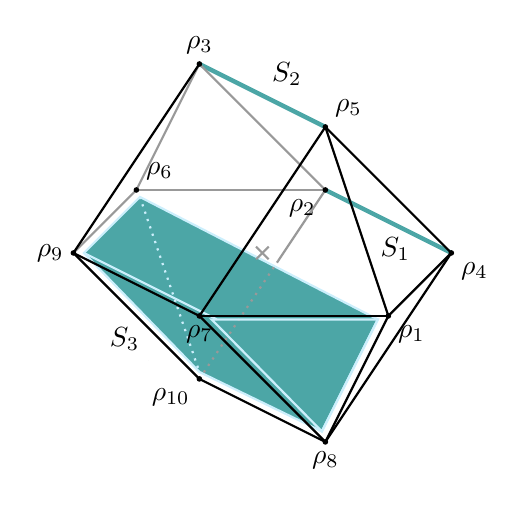
\begin{tikzpicture}[scale=0.8,every node/.style={scale=1}]

\filldraw[color=cyan!20, fill=blue!50!green!70, thick] (-2+1/18,1-2/18) -- (2-3/18,-1-1/18) -- (1-1/18,-3+3/18) -- (-1,-2+2/18) -- (-3+3/18,0) -- cycle; 
\draw[ultra thick, blue!50!green!70] (1,1) -- (3,0);
\draw[ultra thick, blue!50!green!70] (-1,3) -- (1,2);
\draw[thick, dotted, cyan!20] (-2+1/18,1-2/18) --  (-1,-2+2/18);

%background edges
\draw[gray!80, thick] (1,1) -- (-2,1);
\draw[gray!80, thick] (1,1) -- (-1,3);
%\draw[gray!80, thick] (1,1) -- (3,0);
\draw[gray!80, thick] (-1,3) -- (-2,1);
\draw[gray!80, thick] (-3,0) -- (-2,1);
\draw[gray!80, thick] (1,1) -- (1/4,-1/8);
\draw[gray!80, dotted, thick] (1/4,-1/8) -- (-1,-2);
%\draw[gray!80, dashed, thick] (-1,-2) -- (-2,1);

\draw[thick, cyan!20] (2-3/18,-1-1/18) -- (-1+3.5/18,-1-1/18) --   (1-1/18,-3+3/18)  -- cycle;
\draw[thick, cyan!20]  (-3+3/18,0)  -- (-1+5/18,-1-1/18);

%foreground edges
\draw[black, thick] (-3,0) -- (-1,3);
\draw[black, thick] (-3,0) -- (-1,-1);
\draw[black, thick] (-1,-1) -- (1,2);
\draw[black, thick] (1,2) -- (3,0);
\draw[black, thick] (1,2) -- (2,-1);
\draw[black, thick] (-1,-1) -- (2,-1);
\draw[black, thick] (2,-1) -- (3,0);
%\draw[black, thick] (1,2) -- (-1,3);
\draw[black, thick] (3,0) -- (1,-3);
\draw[black, thick] (2,-1) -- (1,-3);
\draw[black, thick] (-1,-2) -- (1,-3);
\draw[black, thick] (-1,-2) -- (-3,0);
\draw[black, thick] (-1,-1) -- (1,-3);

%origin 
\draw[gray!80, thick] (0.1,0.1) -- (-0.1,-0.1);
\draw[gray!80, thick] (-0.1,0.1) -- (0.1,-0.1);


%nodes
\filldraw[black] (2,-1) circle (1pt) node[anchor=north west] {$\rho_1$};
\filldraw[black] (3,0) circle (1pt) node[anchor=north west] {$\rho_4$};
\filldraw[black] (1,1) circle (1pt) node[anchor=north east] {$\rho_2$};
\filldraw[black] (-2,1) circle (1pt) node[anchor=south west] {$\rho_6$};
\filldraw[black] (-3,0) circle (1pt) node[anchor=east] {$\rho_9$};
\filldraw[black] (1,-3) circle (1pt) node[anchor=north] {$\rho_8$};
\filldraw[black] (-1,-2) circle (1pt) node[anchor=north east] {$\rho_{10}$};
\filldraw[black] (1,2) circle (1pt) node[anchor=south west] {$\rho_5$};
\filldraw[black] (-1,3) circle (1pt) node[anchor=south] {$\rho_3$};
\filldraw[black] (-1,-1) circle (1pt) node[anchor=north ] {$\rho_7$};


\filldraw[black] (2.5,0.4) circle (0pt) node[anchor=north east] {$S_1$};
\filldraw[black] (0,2.5) circle (0pt) node[anchor=south west] {$S_2$};
\filldraw[black] (-1.8,-1.7) circle (0pt) node[anchor=south east] {$S_3$};


%\filldraw[black] (5,-3) circle (1pt) node[anchor=north west] {$(1,1,-1)$};
%\filldraw[gray] (2,-2) circle (1pt) node[label={[xshift=-0.9cm, yshift=-0.3cm]\textcolor{black}{$(0,1,-1)$}}]{};
%\filldraw[gray] (-6,-7) circle (1pt) node[label={[xshift=1.3cm, yshift=-0.3cm]\textcolor{black}{$(-1,-2,-2)$}}]{};
%\filldraw[black] (-2,-10) circle (1pt) node[anchor=north] {$(1,-3,-2)$};
%
%\filldraw[gray] (0,-3) circle (1pt) node[anchor=south east]{};
\end{tikzpicture}

\caption{Scaffolding of P735}
\label{ScaffoldingP735}

\end{figure}



Let $\Sigma_Z$ be the normal fan of $S_3$. The rays of $\Sigma_Z$ are the following vectors in $M = \Hom_\ZZ(N, \ZZ)$:
\begin{equation*}
	\begin{aligned}
		v_1 & = (0,-1,0), \\
		v_2 &= (0,0,-1), \\
		v_3 &= (-1,1,1), \\
	v_4 &=	(0,1,1), \\
	v_5 &=	(1,0,0).
	\end{aligned}
\end{equation*}
%which are ordered according to the order of the $2$-faces of $S_3$ in \eqref{eq:2-faces_of_S3}.
%The $3$-dimensional cones of $\Sigma_Z$ are
%\begin{equation*}
%	\begin{gathered}
%		\cone{v_1, v_2, v_3}, \cone{v_2, v_3, v_4}, \cone{v_1, v_3, v_4}, \\
%		\cone{v_2, v_4, v_5}, \cone{v_1, v_2, v_5}, \cone{v_1, v_4, v_5}.
%	\end{gathered}
%\end{equation*}
Let $Z$ be the $T_M$-toric variety associated to the $\Sigma_Z$. It is smooth, projective of dimension $3$. Since $\conv(S_1 \cup S_2 \cup S_3)=P$, the collection $S=\{S_1, S_2, S_3\}$ represents a \textit{scaffolding} of $P$ with shape $Z$, as introduced in \cite{laurent_inversion}. 

%
%For $1 \leq i \leq 5$, let $E_i$ be the torus invariant prime divisor on $Z$ associated to the ray $\cone{v_i}$ in $\Sigma_Z$.
%The divisor sequence
%\begin{equation*}
%	0 \longrightarrow N \longrightarrow \Div_{T_M}(Z) \longrightarrow \Pic(Z) \longrightarrow 0
%\end{equation*}
%of $Z$ is
%\begin{equation*}
%	0 \longrightarrow \ZZ^3 \xrightarrow{\begin{pmatrix}
%			0 & -1 & 0 \\
%			0 & 0 & -1 \\
%			-1 & 1 & 1 \\
%			0 & 1 & 1 \\
%			1 & 0 & 0
%	\end{pmatrix}}
%\ZZ^5
%\xrightarrow{\begin{pmatrix}
%		1 & 1 & 0 & 1 & 0 \\ 
%		1 & 1 & 1 & 0 & 1
%\end{pmatrix}}
%\ZZ^2 \longrightarrow 0
%\end{equation*}
We also see that $Z$ is a $\PP^2$-bundle over $\PP^1$, namely $Z = \PP_{\PP^1} \left( \cO \oplus \cO(1)^{\oplus 2}  \right)$. This ensures that the Laurent inversion construction embeds $X$ as a complete intersection of codimension $\rho(Z)=2$ (see the proof of \cite[Proposition~12.2]{laurent_inversion}). 
In particular, the relations that give the $\PP^2$-bundle structure on $\PP^1$ are 
\begin{equation}
\label{eq:relations}
	\begin{aligned}
		v_1+v_2+v_4 &=0\\
		v_3+v_5&=v_4.
	\end{aligned}
\end{equation}
Here the first relation simply describes the $\PP^2$ fibre, while the second is a primitive relation (in the sense of Batyrev \cite{Batyrev}) obtained by pulling back of the relation $v'_3+v'_5=0$ in the quotient lattice induced by the projection to $\PP^1$. %In particular, the $v_i$ appearing on its right-hand side have positive coefficients (see proof of \cite[Proposition~12.2]{laurent_inversion}). 

Consider the following $3$ torus invariant nef divisors on $Z$:
\begin{equation}
\label{eq:struts}
	\begin{aligned}
		D_1 &= E_1 - E_4, \\
		D_2 &= E_2 - E_4, \\
		D_3 &= E_3 + E_4 + E_5,
	\end{aligned}
\end{equation} 
where $E_i$ are the torus-invariant divisors associated to the $v_i$. Their section polytopes are exactly $S_1$, $S_2$, $S_3$, respectively.

We consider the lattice $\widetilde{N} = \Div_{T_M} Z= \ZZ^5$ with basis $E_1, \dots, E_5$. This will be the ambient lattice for the fan of $Y$ which we describe below as a GIT quotient using the expressions in \eqref{eq:struts}. We then use the relations \eqref{eq:relations} to deduce the equations of $X$ inside $Y$, keeping in mind the correspondence $E_i \leftrightarrow v_i$.

Following the construction in \cite[Algorithm~5.1]{laurent_inversion}, the weight matrix of $Y$ is of size $(r+z)\times r=8\times 3$, where $r$ is the number of $S_i$ and $z$ is the number of rays in $\Sigma_Z$, given by:
\[\begin{matrix}
I_1 &I_2 &I_3& E_1 &E_2 &E_3 &E_4 & E_5\\
\hline 
1 & 0 & 0 & 1 & 0& 0& -1& 0\\
0 &1 &0 &0 &1 &0 &-1& 0\\
0 &0 &1 &0 &0 &1 &1 &1\\
\hline
y_1& y_2& y_3&y_4&y_5&y_6&y_7&y_8
\end{matrix}\]
Here a row $i$ corresponds to a strut $S_i$ (or, alternatively, to a divisor $D_i$ whose polytope is $S_i$) and each $(i,j)$ entry outside of the $r\times r$-identity block is the coefficient of $E_{j}$ in the expression of $D_i$ in \eqref{eq:struts}. 

The equations of $X$ in the Cox coordinates on $Y$ are \[y_4y_5y_7=y_3 \quad \text{and} \quad y_6y_8=y_7y_1y_2y_3,\] which are deduced from \eqref{eq:relations} as explained in \cite[Proposition~12.2]{laurent_inversion}.

%i.e. homogenisations of the equations $t_4t_5t_7=1$ and $t_6t_8=t_7$ on $T_Y$. 

%Indeed, the image of the injective map $N\hookrightarrow \Div_{T_M}(Z)=\widetilde{N}$ is given by the relations in \eqref{eq:relations}, as part of the divisor sequence of $Z$. This induces an injection of tori $T_N\hookrightarrow T_{\widetilde{N}}$ given by $t_4t_5t_7=1$ and $t_6t_8=t_7$ on $T_{\widetilde{N}}$, y_and what  \cite[Theorem~5.5]{laurent_inversion} does is compactify its image to global equations on $Y$ using the remaining coordinates in the identity block $y_1,\ldots, y_3$.

In particular, this shows that $X$ is a complete intersection $L_1\oplus L_2$, where $L_i$ are $(\CC^*)^3$-linearised line bundles with weights
\[
L_1=\cO_Y(y_4)\otimes \cO_Y(y_5)\otimes\cO_Y(y_7)=\cO_Y\begin{pmatrix}0\\0\\1\end{pmatrix}
\]
and
\[
L_2=\cO_Y(y_6)\otimes \cO_Y(y_8)=\cO_Y\begin{pmatrix}0\\0\\2\end{pmatrix}.
\]
According to \cite[Theorem~5.5]{laurent_inversion}, this is an embedding of a Fano variety; a posteriori the stability condition needed to define $Y$ should be chosen such that \[-K_Y-L_1-L_2=\cO_Y\left(\begin{pmatrix}1\\1\\4\end{pmatrix}-\begin{pmatrix}0\\0\\1\end{pmatrix}-\begin{pmatrix}0\\0\\2\end{pmatrix}\right)=\cO_Y\begin{pmatrix}1\\1\\1\end{pmatrix}\] is ample, i.e. $\omega=(1,1,1)$. \end{proof}

\begin{remark}
The ambient space $Y$ thus obtained is in fact a smooth toric $5$-fold. Since the first equation of the embedding in Proposition~\ref{prop:X_inside_Y} is linear in $y_3$, we can solve for this variable and transform the second equation into $y_6y_8=y_7^2y_1y_2y_4y_5$. Up to renaming the ambient Cox variables, this is exactly the embedding of $X$ inside the $4$-fold $F$ from Proposition~\ref{prop:X_inside_F}.
%The stability condition remains unchanged, therefore by adjunction $X$ is still Fano inside $F$.

%Its rays (corresponding to the Cox coordinates $y_1,\ldots, y_8$ respectively) are:
%\begin{equation*}
%		\begin{gathered}
%			\widetilde{\rho_1} = \begin{pmatrix}
%				1 \\ 0 \\ 0 \\ 0 \\ 0 
%			\end{pmatrix}\!, \
%			\widetilde{\rho_2}= \begin{pmatrix}
%				0  \\ 1 \\ 0 \\ 0 \\0
%			\end{pmatrix}\!, \
%			\widetilde{\rho_3} = \begin{pmatrix}
%				0 \\ 0 \\ 1 \\ 0 \\ 0
%			\end{pmatrix}\!, \
%			\widetilde{\rho_4} = \begin{pmatrix}
%				0 \\ 0 \\ 0 \\ 1 \\ 0
%			\end{pmatrix}\!, \
%			\widetilde{\rho_5} = \begin{pmatrix}
%				1\\ -1\\0\\ 1\\ 0
%			\end{pmatrix}\!, \\
%			\widetilde{\rho_6} = - \begin{pmatrix}
%				  0\\ 0 \\ 0 \\ 0 \\ 1
%			\end{pmatrix}\!, \
%			\widetilde{\rho_7} = - \begin{pmatrix}
%				1 \\ 0 \\ 0 \\ 1 \\ 0
%			\end{pmatrix}\!, \
%			\widetilde{\rho_8} = - \begin{pmatrix}
%				-1 \\ 0 \\ -1 \\ -1 \\ -1
%			\end{pmatrix}\!.
%		\end{gathered}
%\end{equation*}
%  Its maximal-dimensional cones are 
%  
%    \[ \begin{gathered}  
%    \widetilde{\sigma}_{ 2 3 4 6 7 } ,\
%     \widetilde{\sigma}_{ 2 3 4 7 8 }, \
%     \widetilde{ \sigma}_{ 2 4 6 7 8 }, \
%     \widetilde{\sigma}_ { 1 3 5 6 7}, \
%    \widetilde{  \sigma}_{ 3 4 5 6 8 }, \\
%    \widetilde{  \sigma}_{ 1 5 6 7 8 }, \
%    \widetilde{  \sigma}_{ 4 5 6 7 8 }, \
%     \widetilde{ \sigma}_{ 1 2 3 7 8 }, \
%   \widetilde{  \sigma}_ { 1 2 6 7 8 }, \
%   \widetilde{  \sigma}_ { 1 2 3 6 7 }, \\
%   \widetilde{   \sigma}_{ 1 2 3 6 8 }, \
%   \widetilde{  \sigma}_ { 1 3 5 7 8 }, \
%    \widetilde{ \sigma}_ { 1 3 5 6 8 }, \
%    \widetilde{  \sigma}_{ 3 4 5 6 7 }, \
%    \widetilde{  \sigma}_{ 2 3 4 6 8 }, \
%    \widetilde{  \sigma}_{ 3 4 5 7 8 }.
%      \end{gathered}\]
\end{remark}



%
%\begin{prop}
%
%Let $F$ be the toric $4$-fold ...
%Then $X$ can be embedded into $F$ as the zero-section of a section of $L^{\otimes 2}$, where $L$ is the $(\CC^*)^3$-linearised line bundles on $F$ of weights $(0,0,1)$.
%More specifically, the equation of $X$ in the Cox coordinates of $F$ is
%\[x_6x_3=x_7^2x_1x_2x_4x_5\] 
%and the equation of a smoothing of $X$ is given by a general section of $L^{\otimes 2}$:
%\begin{align*}   x_1x_3x_5x_7+   x_1x_5x_6x_7+    x_1^2x_2^2x_7^2+    x_1x_2x_4x_5x_7^2+    x_4^2x_5^2x_7^2+\\ x_2x_3x_4x_7+    x_2x_4x_6x_7+    x_2^2x_4^2x_7^2+    x_1^2x_2x_5x_7^2+    x_1x_4x_5^2x_7^2+ \\   x_1x_2x_3x_7+    x_1x_2x_6x_7+    x_3x_4x_5x_7+    x_4x_5x_6x_7+    x_6^2+ \\  x_1x_2^2x_4x_7^2+    x_2x_4^2x_5x_7^2+    x_3^2+    x_3x_6+    x_1^2x_5^2x_7^2&=0 \end{align*}
%\end{prop}
%Note that when writing the above equation, we use the following coefficient convention: when writing, every monomial appears with coefficient one, yet this signifies that each monomial is assigned a random coefficient (that is, independent from the others).
%
%




%Consider the dual $\widetilde{M} = \Hom_\ZZ (\widetilde{N}, \ZZ)$.  
%Let $\langle \cdot, \cdot \rangle \colon \widetilde{M}_\RR \times \widetilde{N}_\RR \to \RR$ be the duality pairing.
%Consider the polytope $Q \subseteq \widetilde{M}_\RR$ defined by the inequalities:
%\begin{equation*}
%	\begin{aligned}
%		\langle \cdot, -D_1 \rangle &\geq -1, \\
%				\langle \cdot, -D_2 \rangle &\geq -1, \\
%						\langle \cdot, -D_3 \rangle &\geq -1, \\
%			\langle \cdot, E_1 \rangle &\geq 0, \\
%			\langle \cdot, E_2 \rangle &\geq 0, \\
%			\langle \cdot, E_3 \rangle &\geq 0, \\
%			\langle \cdot, E_4 \rangle &\geq 0, \\
%						\langle \cdot, E_5 \rangle &\geq 0. \\
%	\end{aligned}
%\end{equation*}
%The polytope $Q$ is $5$-dimensional, has $16$ vertices and $8$ facets.
%
%Let $\Sigma_Y$ be the normal fan of $Q$.
%The primitive generators of the rays of $\Sigma_Y$ are $-D_1$, $-D_2$, $-D_3$, $E_1$, $E_2$, $E_3$, $E_4$, $E_5$.
%Let $Y$ be the toric variety associated to $\Sigma_Y$; it is a smooth Fano $5$-fold.
%

%Starting from the embedding constructed in Proposition~\ref{prop:X_inside_Y} we construct an embedding of the toric Fano $3$-fold considered in Proposition~\ref{prop:definition_P_X} into a toric $4$-fold.

%\begin{proof}
%We solve the first equation in Proposition~\ref{prop:definition_P_X} for $y_3$ and in order to minimally disrupt notation we denote the coordinate $x_8$ on $Y$ by $x_3$ on $F$ (this changes nothing geometrically). We obtain $X$ as a hypersurface in this new ambient space with only the second equation remaining. 
%
%Denote by $\bar{X}$ the variety given by the general equation, which is by construction a $\QQ$-Gorenstein deformation of $X$. It remains to check that $\bar{X}$ is smooth. An elementary computer verification shows that $\bar{X}\subset F$ is quasi-smooth, i.e. the irrelevant ideal of $F$ is a sub-ideal of the jacobian ideal of the general section. This implies that $\bar{X}$ can at most inherit singularities from its ambient space $F$. But, similarly to $Y$, $F$ is smooth, therefore so is $\bar{X}$. A posteriori, $\bar{X}$ is also well-formed (in dimension three this is equivalent to having isolated singularities), so we can apply the usual adjunction formula to determine that $-K_{\bar{X}}=(1,1,1)$, which is ample, therefore we have constructed a smooth Fano variety.
%
%\end{proof}







\bibliography{Biblio_Liana_Andrea}



\end{document}
